\chapter{SMPC Protocols for Secure Differentially Private Mechanisms}
\label{cha:MPCProtocolsforDifferentiallyPrivateMechanisms}

In this chapter, we first present the SMPC-DP procedure that combines \smpc and differentially private mechanisms.
% We first give a general overview of the settings and description of our SMPC-DP procedure.
Then, we construct the \smpc protocols for the previously introduced secure differentially private mechanisms and noise sampling algorithms (cf.~\autoref{cha:secureDPMechanisms}).

Generally, we face two technical challenges when transforming the differentially private mechanisms into \smpc protocols.
The first is to identify the most efficient \smpc protocols for arithmetic operations.
The second is to determine the most efficient sampling algorithms for differentially private mechanisms in \smpc.
For the first challenge, we implement \smpc protocols that support (signed) integer arithmetic, fixed-point arithmetic, floating-point arithmetic, and data type conversions in MOTION~\cite{braun2022motion} and compare their performance in~\autoref{sec:ArithmeticOperationsPerformanceEvaluation}.
For the second challenge, we construct the \smpc protocols for the all previously introduced noise sampling algorithms and compare their performance in \autoref{sec:DifferentiallyPirvateMechanismBenchmarks}.

\textbf{SMPC-DP Procedure Overview.}
In our SMPC-DP procedure, we consider $n$ users, $N$ computation parties and one reconstruction party as \autoref{img:MPCDPProcedure} shows.
The SMPC-DP procedure consists of three steps:
(i) The users $U_i$ send the secret shared data $\left\langle D_i\right\rangle $ to the computation parties.
(ii) The computation parties execute the \smpc protocols to compute function $\left\langle f\left(D_1,\ldots, D_n\right) \right\rangle $, generate secret shared noise $\left\langle noise\right\rangle $, and perturb $\left\langle f\left(D_1,\ldots, D_n\right) \right\rangle $.
(iii) The computation parties send their share of the perturbed result $\left\langle f\left(D_1,\ldots, D_n\right) +noise\right\rangle$ to the reconstruction party, that reconstructs the perturbed result $f\left(D_1,\ldots, D_n\right) +noise$.
% \textbf{Setting.}
%  Each user $P_i$ has private data $D_i$. The computation parties $C_i$ help the users to compute a function $f$ with the distributed data $\left(D_1,\ldots, D_n\right) $ and perturb the result. 
The reconstruction party could be one of the computation parties. We assume that the communication channels between users and computation parties are secure and authenticated, and the communication channels between computation parties are pair-wise secure and authenticated. The users can go offline after sending their secret shared private data $\left\langle D_i\right\rangle $ to the computation parties.

\textbf{Privacy Goals.}
For users, computation parties, and the reconstruction party, the reconstructed perturbed result $f\left(D_1,\ldots, D_n\right) +noise$ should satisfy differential privacy, and the whole computation process leak no information about the individual users' private data $D_i$.

\textbf{Attacker Model.}
% The users, computation parties, and the reconstruction party may be corrupted and collude with each other.
% We assume that the users honestly secret share their private data to the computation parties. 
% For the computation parties, we assume that the adversaries are semi-honest (i.e., they follow the protocol specifications but try to infer information), and there is at least one computation party that is not corrupted (i.e., full-threshold security). 
Since MOTION~\cite{braun2022motion} is secure against $N-1$ semi-honest corruptions, we assume that the computation parties are semi-honest, and there is at least one computation party that is not corrupted.
% Other \smpc protocols (e.g., secure again malicious adversaries (ref.???)) could also be applied in our SMPC-DP procedure but may be less efficient.
% \section{General Procedure for Combining \smpc and DP}
% \label{sec:ProcedureMPCDP}

\begin{figure}[htbp]
      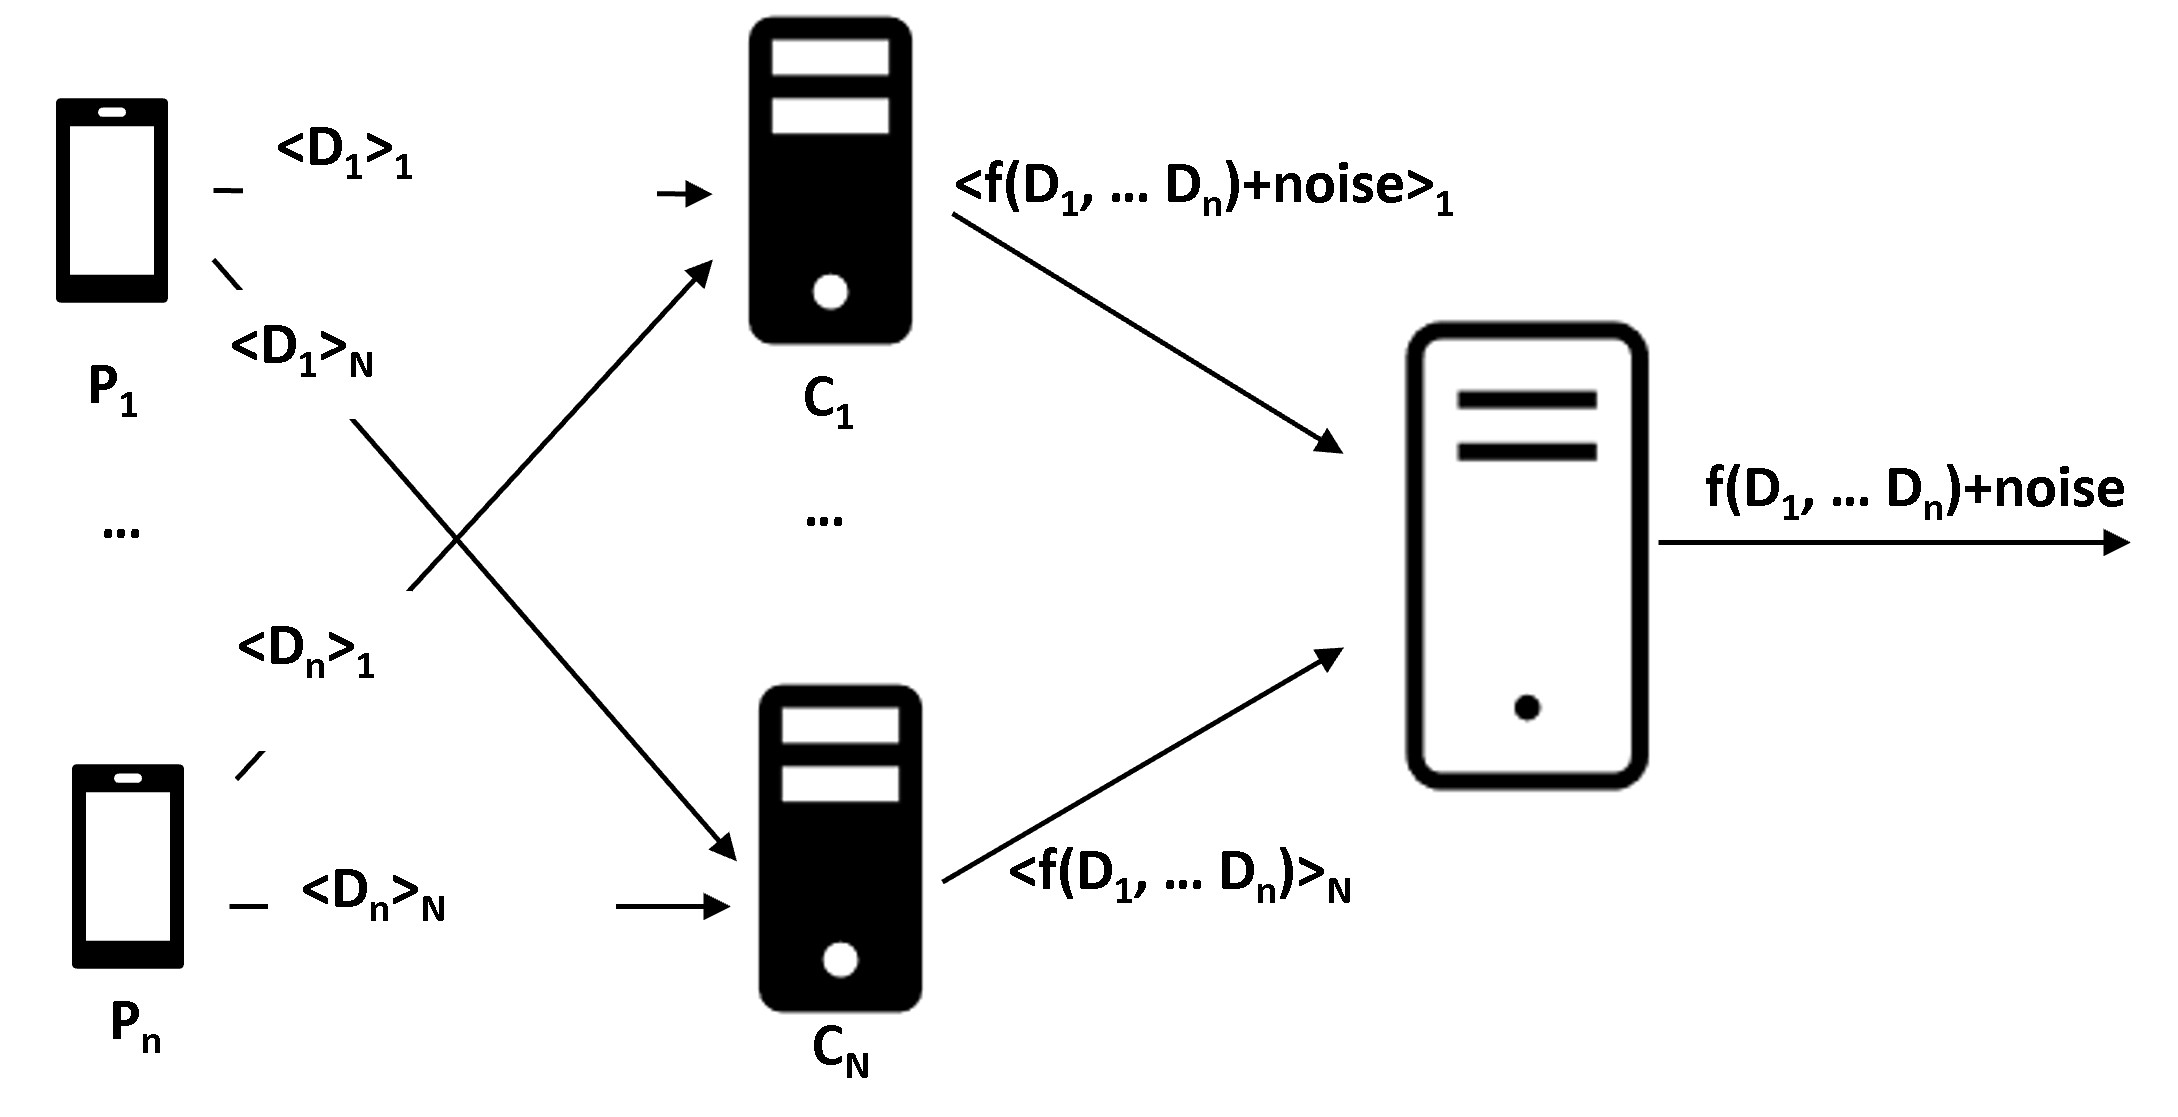
\includegraphics[width=\textwidth]{SMPC-DP procedure}
      \centering
      \caption{SMPC-DP procedure}
      \label{img:MPCDPProcedure}
\end{figure}
\FloatBarrier



% The users first secret share their private data $\left\langle D_i\right\rangle $ to the computation parties, and then, the computation parties compute $\left\langle f\left(D_1,\ldots, D_n\right) \right\rangle $, perturb the result, and send it to the reconstruction party.

% In the following parts, we first describe the \smpc building block, arithmetic operations, and the five \smpc protocols of the previous introduced differentially private mechanisms (cf.~\autoref{cha:secureDPMechanisms}).


% % Let dataset $D=\left( D_{1},\ldots, D_{n}\right) $ be distributed among $n$ parties $\left( P_{i}\right) _{i\in \left[ n\right] }$ who do not trust each other and party $P_{i}$ owns data $D_{i}$. The parties $\left(P_{i}\right)_{i \in \left[ n\right]} $ wish to jointly compute a public function $f$ on their private inputs $\left(pre\left(D_i\right)\right)_{i \in \left[ n\right]} $. After the computation, \CHANGED{either all parties or designated parties receive the result of $f\left(pre\left(D_1\right),\ldots,pre\left(D_n\right)\right)$ as output}, where $pre$ is a pre-processing function executed on their local data $\left(D_i\right)_{i \in \left[ n\right]} $. The parties want to achieve (1) computational privacy (i.e., each party's input is kept secret), \CHANGED{(2) output privacy (i.e., the output satisfies the DP),} and (3) obtain a result with reasonable accuracy.
% % \begin{enumerate}
% % 	\item The computation of $f$ should reveal nothing but the result.
% % 	\item The computation result of $f\left(pre\left(D_1\right),\ldots,pre\left(D_N\right)\right)$ should be identical to the scenario, where a trusted server has access to the whole dataset $D$ and computes $f\left( pre\left(D\right) \right)$ locally, i.e., $f\left(pre\left(D_1\right),\ldots,pre\left(D_N\right)\right)=f\left( pre(D)\right)$.
% % 	\item The result has to satisfy the differential privacy by adding it with noise, i.e., an adversary cannot infer too much information from the noisy result.
% % 	\item The noisy result can still provide statistically useful information.
% % \end{enumerate}

% % To achieve computational privacy, the parties deploy a \smpc protocol $\Uppi^{f}$ which takes $\left(pre\left(D_i\right)\right)_{i \in \left[ n\right]} $ as input and reveals only the computation result. For requirements (2) and (3), we design a SMPC-DP procedure (cf.~\autoref{prot:SMPC-DP}) which combines $\Uppi^{f}$ with a secure differentially private mechanism. Note that in following, we omit the data pre-processing procedure $pre\left(\cdot\right) $ for simplicity and use $f\left( D\right)$ to represent $f\left(D_1,\ldots,D_n\right)$.

% % Let's consider a trival example that combines \smpc protocols with a differentially private mechanism. Suppose the parties $\left(P_{i}\right)_{i \in \left[ n\right]} $ wish to calculate the sum of their local data $\left(D_{i}\right)_{i \in \left[ n\right]} $ with a publicly known function $f\left(D_1,\ldots,D_n\right)=\sum_{j=1}^{n} D_j$, and $f$ has $\ell_2$-\textit{sensitivity} $\Delta^{\left(f\right) } _2=1$ (cf.~\autoref{def:sensitivity}). Meanwhile, the parties require that only the computation result of $f$ should be revealed and differential privacy must be satisfied. To achieve this, each party first adds noise $r_i$ to its local data $D_i$ and determines $ y_{i}=D_{i} +r_{i}$. Recall that in \autoref{def:gaussianMechanism}, we have showed that $ y_{i}=$ satisfies $\left(\varepsilon ,\delta \right) $-DP for $r_i \sim \mathcal{N}\left( 0,\sigma ^{2}\right) $, where $\sigma ^{2}=\frac{2}{\varepsilon ^2}\cdot\ln\left(\frac{1.25}{\delta }\right)$ and $i\in \left[n\right] $. Then, the parties jointly run the \smpc protocol $\Uppi^{f}$ with their private inputs $y_i$ to compute function $f$. After reconstruction they get $y=\sum_{j=1}^{n} y_j=\sum_{j=1}^{n}\left( D_j+ r_j\right)$. Because of the infinite divisibility of the normal distribution~\cite{patel1996handbook}, we have $\sum_{j=1}^{n} r_j \sim \mathcal{N}\left( 0,\sigma_{sum} ^{2}\right) $ for $\sigma_{sum} ^{2}=\sum ^{n}_{j=1}\sigma ^{2}$. Therefore, the computation result $y$ satisfies $\left(\frac{\varepsilon}{\sqrt{n}},\delta \right) $-DP.

% % In general, the parties in above example can achieve $\left(\frac{\varepsilon}{\sqrt{n}},\delta \right) $-DP assuming no corrupted parties. However, in realistic scenarios, corrupted parties may try to extract information of certain parties by weaking the achieved differential privacy protection level.
% % After executing aforementioned steps honestly and obtaining the computation result $y$, the corrupted parties subtract the noise they have added from $y$. In the worst case, i.e., $n-1$ parties are corrupted, the differential privacy guarantee reduces from $\left(\frac{\varepsilon}{\sqrt{n}},\delta \right) $-DP to $\left(\varepsilon,\delta \right) $-DP. If, however, having $\left(\frac{\varepsilon}{\sqrt{n}},\delta \right) $-DP is required, a potential naive solution is that each party adds \textit{more} noise, .e.g, $r_i^{\prime} \sim \mathcal{N}\left( 0,n\cdot \sigma ^{2}\right) $, locally before running $\Uppi^{f}$. However, \CHANGED{this can lead to a severely accuracy reduction}.

% % To summarize, a well-designed SMPC-DP procedure requires a more careful integration of \smpc protocols and differentially private mechanisms. \CHANGED{To guarantee the both the accuracy and privacy, we define several requirements, that is based on the "ideal scenario" with a centralized data server, i.e., a trusted server that has access to all the parties' data $D$ locally computes $f\left( D\right) $ before adding an essential amount of noise to guarantee DP}:

% % \begin{enumerate}
% % 	\item The SMPC-DP procedure should achieve the same privacy protection level as in the centralized data server scenario, and the amount of noise $r$ (in above example: $r=\sum_{j=1}^{n} r_j$) should \CHANGED{exactly match that of the centralized data server scenario}.
% % 	\item The DP guarantee of the SMPC-DP procedure should not degenerate in the presence of corrupted parties.
% % \end{enumerate}

% % \textbf{SMPC-DP Procedure} It can be used among $n$ parties, or in an outsourcing scenario, i.e., an arbitrary amount of parties secret share their private inputs to $N$ ($N\ll n$) non-colluding computing parties. Then, the computing parties execute the $N$-party SMPC-DP protocol, where they compute $f$ and add noise shares to get the noisy secret-shared results. Finally, the noisy secret-shared results are sent back to the parties for reconstruction. We assume semi-honest adversaries that follow the protocol specifications but wish to infer additional information\cite[Chapter 2]{evans2017pragmatic}.

% % Specifically, for $i\in \left[ n\right]$, party $P_{i} $ secret shares his inputs $D_i$ to $N$ computing parties $P_{0},\ldots,P_{N}$. For $j\in \left[ N\right]$, computing party $P_j$ runs \smpc protocols for function $f$ with other computing parties using his secret-shared value $\left\langle D_1 \right\rangle _{j},\ldots,\left\langle D_n \right\rangle _{j} $ (received from $n$ parties) and get $\left\langle f\left(D\right) \right\rangle _j$. Then, computing party $P_j$ runs the \smpc protocols for distributed noise generation (DNG) with other computing parties and get a secret-shared noise $\left\langle r\right\rangle_j $. Finally, computing party $P_j$ perturbs $\left\langle f\left(D\right) \right\rangle _j$ by computing $\left\langle M\left(D\right)\right\rangle_j=\Uppi^{Perturbation}\left(\left\langle f\left(D\right) \right\rangle_j+\left\langle r\right\rangle_j\right) $ and sends it to the parties responsible for the reconstruction. Note that during the distributed noise generation, each computing party only gets a secret-shared noise $\left\langle r\right\rangle $ and even $N-1$ colluding computing parties cannot reconstruct the noise $r$. After the reconstruction, only the perturbed (noisy) result $M\left(D\right)=\text{Perturb}\left(f\left(D\right)+r\right)  $ is revealed which computes function $f$ and guarantees differential privacy. More important is that we prevent excessive noise and ensure utility since the noise $r$ is generated by all the parties instead of by each party independently (as in the above example).


% % ~\autoref{prot:SMPC-DP} describes outsourcing scenario of the SMPC-DP procedure. Note that the parties calculate $\left\langle f\left(D\right)\right\rangle =\Uppi^{f }\left(\left\langle D_1 \right\rangle ,\ldots,\left\langle D_n \right\rangle\right) $ and add the securely generated noise $\left\langle r\right\rangle$ (output perturbation) to guarantee DP. In this work, we assume that each party has computed $\left\langle f\left(D\right) \right\rangle$ and focus on the process of $\Uppi^{Noise }$, i.e., distributed noise generation (DNG).

% % \begin{protocol}[tbh!]
% % 	\centering
% % 	\fbox{
% % 		\pseudocode[space=none, syntaxhighlight=auto, addkeywords={Protocol, Input, Output},linenumbering, skipfirstln, head=\textbf{Protocol: $\Uppi^{SMPC-DP}\left(\left\langle D_1 \right\rangle ,\ldots,\left\langle D_n \right\rangle\right) $}]{
% % 			\textbf{Input: $\left\langle D_1 \right\rangle ,\ldots,\left\langle D_n \right\rangle$ } \pcskipln \\
% % 			\textbf{Output: $\left\langle M\left(D\right)\right\rangle=\left\langle f\left(D\right) \right\rangle +\left\langle r\right\rangle$} \\
% % 			\text{$\left\langle f\left(D\right)\right\rangle \gets \Uppi^{f }\left(\left\langle D_1 \right\rangle ,\ldots,\left\langle D_n \right\rangle\right) $.}\\
% % 			\text{$\left\langle r\right\rangle \gets \Uppi^{Noise } $}\\
% % 			\text{$\left\langle M\left(D\right)\right\rangle\gets \Uppi^{Perturb}\left(\left\langle f\left(D\right) \right\rangle,\left\langle r\right\rangle\right) $}
% % 		}}
% % 	\caption{SMPC-DP procedure.}
% % 	\label{prot:SMPC-DP}
% % \end{protocol}
% % \FloatBarrier



\section{Building Blocks}
\label{sec:MPCBuildingBlocks}
We construct \smpc protocols based on the following building blocks (details can be found in \autoref{app:MPCBuildingBlocks}):

\begin{enumerate}

      % \item $\left\langle \boldsymbol{y}\right\rangle^B \gets \Uppi^{RandBits}\left(\ell\right) $ allows parties to generate shares of a publicly unknown random $\ell$-bit string $\left\langle \boldsymbol{y}\right\rangle^B =\left( \left\langle y_{0}\right\rangle^B ,\ldots ,\left\langle y_{\ell-1}\right\rangle ^B\right)$ without interactive operation. Specifically, each party

      % \item $\left\langle \boldsymbol{y}\right\rangle^B \gets \Uppi^{PreOr}\left(\left\langle \boldsymbol{x}\right\rangle ^B\right) $ computes the prefix-OR of an $\ell$-bit string $\left\langle \boldsymbol{x}\right\rangle^B= \left(\left\langle x_{0}\right\rangle ^B,\ldots, \left\langle x_{\ell-1}\right\rangle ^B\right) $ and output $\left\langle \boldsymbol{y}\right\rangle^B= \left(\left\langle y_{0}\right\rangle ^B,\ldots, \left\langle y_{\ell-1}\right\rangle ^B\right) $ such that $\left\langle y_{j}\right\rangle^B = \lor _{k=0}^{j} \left\langle x_{k} \right\rangle ^B$ for $j \in \left[0,\ell-1\right] $, where $\left\langle y_{0}\right\rangle^B =\left\langle x_{0} \right\rangle ^B$.
      \item $\left\langle \boldsymbol{y}\right\rangle^B \gets \Uppi^{PreOr}\left(\left\langle \boldsymbol{x}\right\rangle ^B\right) $ computes the prefix-OR of an $\ell$-bit string $ \boldsymbol{x}= \left( x_{0},\ldots,  x_{\ell-1}\right) $ and output $\left\langle \boldsymbol{y}\right\rangle^B= \left(\left\langle y_{0}\right\rangle ^B,\ldots, \left\langle y_{\ell-1}\right\rangle ^B\right) $ such that $ y_{j} = \lor _{k=0}^{j}  x_{k} $ for $j \in \left[0,\ell-1\right] $, where $ y_{0} = x_{0} $.

      \item $\left\langle \boldsymbol{y}\right\rangle^{B} \gets \Uppi^{Geometric} $ generates shares of a geometric random variable $y\sim Geo\left(p=0.5\right) $ using \autoref{algo:Geometric}.

            % which is inspired by the OT-based multiplication algorithms~\cite{asharov2018privacy,schneider2019episode}. For example, in two-party computation, $\left\langle \boldsymbol{x}\right\rangle ^B \cdot \left\langle b\right\rangle ^B$ can be reformulated as follows:
            %       \begin{equation}
            %           \begin{split}
            %               \left\langle \boldsymbol{x}\right\rangle ^B \cdot \left\langle b\right\rangle ^B &=\left(\left\langle \boldsymbol{x}\right\rangle ^B_0\oplus \left\langle \boldsymbol{x}\right\rangle ^B_1\right)  \cdot \left(\left\langle b\right\rangle ^B_0 \oplus \left\langle b\right\rangle ^B_1 \right) \\
            %               &=\left\langle \boldsymbol{x}\right\rangle ^B_0 \cdot \left\langle b\right\rangle ^B_0 \oplus  \left\langle \boldsymbol{x}\right\rangle ^B_0 \cdot \left\langle b\right\rangle ^B_1  \oplus \left\langle \boldsymbol{x}\right\rangle ^B_1 \cdot \left\langle b\right\rangle ^B_0 \oplus  \left\langle \boldsymbol{x}\right\rangle ^B_1 \cdot \left\langle b\right\rangle ^B_1 ,
            %           \end{split}
            %       \end{equation}
            %       where $\left\langle \boldsymbol{x}\right\rangle ^B_0 \cdot \left\langle b\right\rangle ^B_0$ and $\left\langle \boldsymbol{x}\right\rangle ^B_1 \cdot \left\langle b\right\rangle ^B_1$ can be calculated by each party locally. For the remaining two mulitplications, we utilize two C-OTs (cf.~\autoref{subsubsec:OT}). For $i \in \left\{0,1\right\} $, $P_i$ inputs $\left\langle b\right\rangle ^B_i$, and $P_{1-i}$ inputs $\left(r_i, r_i\oplus \left\langle \boldsymbol{x}\right\rangle ^B_{1-i} \right) $ and receives $r_i\oplus \left(\left\langle b\right\rangle ^B_i \cdot \left\langle \boldsymbol{x}\right\rangle ^B_{1-i}\right) $, where $r_i$ is a random bit string. Finally, $P_i$ set $r_i \oplus  r_{1-i}\oplus \left(\left\langle b\right\rangle ^B_{1-i} \cdot \left\langle \boldsymbol{x}\right\rangle ^B_{i}\right)$ as its share of $\left\langle \boldsymbol{x}\right\rangle ^B_0 \cdot \left\langle b\right\rangle ^B_1  \oplus \left\langle \boldsymbol{x}\right\rangle ^B_1 \cdot \left\langle b\right\rangle ^B_0 $. We also extend $\Uppi^{OTMult}$ to multiple parties using similar C-OT based approach. We set $\Uppi^{OTMult}$ as default \smpc protocol to compute bit-vector multiplication.
            %       \TODO{check if MOTION has implemented bit-vector multiplication}

            % \item $\left(\left\langle y_1\right\rangle^B,\ldots,\left\langle y_{\ell}\right\rangle^B \right)\gets\Uppi^{Binary2Unary}\left(\left\langle \boldsymbol{x}\right\rangle ^{B},\ell\right) $~\cite{aliasgari2012secure} converts an unsigned integer $x$ from binary to unary bitwise representation and outputs an $\ell$-bit string $\boldsymbol{y}=\left( y_{0} ,\ldots , y_{\ell-1} \right) $, where the $x$ least significant bits $ y_{0} ,\ldots , y_{x-1} $ are set to $1$ and the rest bits $ y_{x} ,\ldots , y_{\ell-1} $ are set to $0$.
            % We use HyCC compiler (cf.~\autoref{subsection:MOTIONFramework}) to generate both the size-optimal and depth-optimal circuit for $\operatorname{AND}$ gate.

            % \item For signed ($INT$) and unsigned integer ($UINT$) operations (e.g., comparison, addition, substraction), we use depth-optimized circuits generated with HyCC (cf.~\autoref{subsection:MOTIONFramework}).

            % \item For floating-point operations, we use the Boolean circuits of work~\cite{demmler2015aby}.

      \item $\left\langle {y}\right\rangle ^{B,UINT}\gets \Uppi^{HW}\left(x_0,\ldots,x_{\ell}\right) $~\cite{boyar2008tight} computes the Hamming weight (i.e., the number of $1$ bits) of an $\ell$-bit string $x_0,\ldots,x_{\ell}$.
            % We first convert the input into Yao's sharing and finally convert the result back to the Boolean sharing.
            %   \TODO{better methods without share conversion???}

      \item $\left\langle \boldsymbol{y_i}\right\rangle ^{B}\gets \Uppi^{ObliviousSelection}\left(\left\langle \boldsymbol{y_0}\right\rangle^{B} ,\ldots,\left\langle \boldsymbol{y_{\ell-1}}\right\rangle^{B},\left\langle c_0\right\rangle ^B,\ldots,\left\langle c_{\ell-1}\right\rangle ^B\right) $ outputs the bit-string $\left\langle \boldsymbol{y_i}\right\rangle ^B$, where $i$ is the index of the first non-zero bit $c_{i}$ for $i\in \left[0,\ell-1\right] $. If all the bits $c_0, \ldots, c_{\ell-1}$ are zeros, bit-string $\boldsymbol{y_i} $ is set to a bit-string consisting of all zeros.

      \item $\left\langle {y}\right\rangle ^{B,UINT} \gets \Uppi^{RandInt}\left(m\right) $ generate shares of a random integer $y$ in the interval $ \left[0,m-1\right] $.

      \item $\left\langle \boldsymbol{y}\right\rangle^B \gets \Uppi^{COTMult}\left(\left\langle \boldsymbol{x}\right\rangle ^B,\left\langle b\right\rangle ^B\right) $~\cite{asharov2018privacy,schneider2019episode} computes the multiplication of a bit string $ \boldsymbol{x}$ and a single bit $ b$ with \correlatedot (cf.~\autoref{subsubsec:OT}).

      \item $\left\langle \boldsymbol{y}\right\rangle ^B \gets  \Uppi^{MUX}\left(\left\langle a\right\rangle^B, \left\langle \boldsymbol{x_0}\right\rangle^B ,\left\langle \boldsymbol{x_1}\right\rangle^B  \right) $ outputs a bit-string $\left\langle \boldsymbol{y}\right\rangle^{B} $, where $ \boldsymbol{y}=\boldsymbol{x_0} $ if $a=1$, $\boldsymbol{y}=\boldsymbol{x_1} $ otherwise.

\end{enumerate}

\section{Number Representations}
\label{sec:NumberRepresentationsandArithmeticOperations}
In \smpc, we use \booleanGMW and \arithmeticGMW protocols to implement arithmetic operations. We consider integers, fixed-point numbers, and floating-point numbers to represent the numbers in the arithmetic operations.
% We discuss the details about implementing these arithmetic operations in MOTION~\cite{braun2022motion}.
% At a high level, we use HyCC~\cite{buscher2018hycc} and CBMC-GC~\cite{buscher2016compiling} to generate depth-optimized circuits or use the available circuits from works~\cite{demmler2015aby,archer2021cost} to implement the \booleanGMW based arithmetic operations. For \arithmeticGMW based arithmetic operations, we extend the arithmetic sharing operations of MOTION~\cite{braun2022motion} to support comparison, shifting, truncation, modulo reduction, etc.

% Further, our \smpc protocols use integer, fixed-point and floating-point arithmetic interchangeably to achieve the best \smpc performance (regarding the communication and computation cost).

\paragraph{BGMW Signed/Unsigned Integer.}
The MOTION framework~\cite{braun2022motion} supports \booleanGMW unsigned integer arithmetic operations, such as $+$, $-$, $*$, $/$, and $<$. We extend it to support other arithmetic operations, e.g., modulo reduction and conversion operations with \booleanGMW fixed-point and \booleanGMW floating-point.
We also extend MOTION~\cite{braun2022motion} to support \booleanGMW signed integers with additional operations such as absolute value and negation.

% We generate depth-optimized binary circuits for \booleanGMW-based unsigned integer with HyCC~\cite{} and CBMC-GC~\cite{}.
% Except for the arithmetic operations supported by the unsigned integer, we also implement signed integer arithmetic that supports operations such as absolute value and negation.

\paragraph{BGMW Floating-Point.}
% We consider 64-bit floating-point arithmetic~\cite{IEEE754_2019}. For operations such as $+,$ $-$, $*$, $/$, $<$, square, square root, exp2, and log2, we use the binary circuits from ABY~\cite{demmler2015aby}. For other operations such as conversion operations with fixed-point and integers, ceil, floor, absolute value, round to the nearest integer, we use CBMC-GC to generate depth-optimized and size-optimized binary circuits with the C code from Berkeley SoftFloat library~\cite{BerkelySoftFloat}.
We consider $64$-bit floating-point arithmetic. For operations such as $+,$ $-$, $*$, $/$, $<$, square, square root, exp2, and log2, we use the binary circuits from ABY~\cite{demmler2015aby}. For other operations such as conversion operations with \booleanGMW fixed-point and \booleanGMW integers, ceil, floor, absolute value, round to the nearest integer, we use CBMC-GC~\cite{buscher2016compiling} to generate depth-optimized binary circuits with the C code from Berkeley SoftFloat library~\cite{BerkelySoftFloat}.

\paragraph{AGMW Floating-Point.}
\label{para:AGMWFloating-Point}
We implement the \arithmeticGMW floating-point protocols primarily based on the work of Aliasgari et al.~\cite{aliasgari2012secure}.
A floating-point number $u$ is represented as a quadruple $\left(v, p, z, s\right) $, where each term is defined as follows:
\begin{enumerate}
      \item $v\in \left[2^{\ell-1},2^{\ell}\right) $ is an $\ell$-bit mantissa (with the most significant bit always set to one),
      \item $p\in \mathbb{Z} _k$ is a $k$-bit signed exponent,
      \item $z\in \left\{0,1\right\} $ is the zero bit that is set to $1$ when $u=0$,
      \item $s\in \left\{0,1\right\}$ is the sign bit of $u$.
\end{enumerate}
This quadruple $\left(v, p, z, s\right) $ represents the value $u= \left(1-2s\right) \cdot \left(1-z\right) \cdot v \cdot 2^p$.
The \smpc protocols for floating-point in work~\cite{aliasgari2012secure} rely on the Shamir secret sharing~\cite{shamir1979share} operations performed over a prime field $\mathbb{F}_p$ (modulo $p$), whereas the arithmetic sharing operations in MOTION~\cite{braun2022motion} are performed in a ring (modulo $\mathbb{Z} _{2^{n}}$). One significant difference between finite field and ring is that there is no inverse element (i.e., $a^{-1}$ in a prime field) in the ring. The inverse operations in the work~\cite{aliasgari2012secure} are primarily for computing the logical right shifting of the shares.
Therefore, we replace the protocols that involve inverse operations in the work~\cite{aliasgari2012secure} with the \smpc protocols that support arithmetic sharing operations (e.g., logical/arithmetic right shifting, modulo reduction, etc.) over a ring from the works~\cite{escudero2020improved,dalskov2020secure,makri2021rabbit}.

\paragraph{BGMW Fixed-Point.}
% We implement fixed-point arithmetic with two precision modes:
% (i) 64-bit fixed-point with a $16$-bit fractional part,
% (ii) 64-bit fixed-point with a $31$-bit fractional part.
We implement fixed-point numbers with a $48$-bit signed integer part and a $16$-bit fractional part.
This gives us precision $2^{-16}$ and covers the values with a integer part up to $47$ bits.
We use HyCC~\cite{buscher2018hycc} to generate the depth-optimized circuits for fixed-point operations, such as $+$, $-$, $*$, $/$, and $<$.
For operations such as exp2 and log2, we use polynomial approximations~\cite{hart1978computer,aly2019benchmarking} and generate corresponding binary circuits using CBMC-GC~\cite{buscher2016compiling}.
For operations such as square root, we use both polynomial approximations~\cite{hart1978computer} and Goldschmidt approximations~\cite{markstein2004software,aly2019benchmarking}.
The main issue with fixed-point arithmetic is the inherent precision loss during arithmetic operations.
We estimate the accuracy of fixed-point exp2 operation by comparing its result to the floating-point exp2 operation with the same input.
For $1000$ random inputs in $\left[0,1\right]$, the absolute error between the fixed-point exp2 operation results and floating-point exp2 operation results are $10^{-4}\approx 2^{-13}$ in average.
% To estimate the accuracy of the fixed-point operations, we sample $1000$ values in a specific range and compare the fixed-point operation result with the floating-point operation result.
% For example, we compute the fixed-point exp2 operation with $1000$ randomly sampled values in $\left[0,1\right] $, the absolute error between fixed-point results floating-point results are $10^{-4}\approx 2^{-13}$ in average.
For log2 (with $1000$ samples in $\left[0.5,1\right] $), the absolute error is $10^{-4}\approx 2^{-13}$, and for the square root operation with polynomial or Goldschmidt approximation, the absolute error is $10^{-4}\approx 2^{-13}$.

\paragraph{AGMW Fixed-Point.}
\label{para:AGMWFixed-Point}
We implement the \arithmeticGMW fixed-point protocols primarily based on the work of Catrina and Saxena~\cite{catrina2010secure}. A fixed-point number $x$ is represented as $x = \overline{x}\cdot  2^{-f}$, where $\overline{x}$ is an $k$-bit signed integer and $f$ is the length of the fractional part.
% Specifically, $\overline{x}\in \mathbb{Z} _{\left\langle k\right\rangle }$ and $ \mathbb{Z} _{\left\langle k\right\rangle }=\left\{x\in \mathbb{Z}  \,|\,-2^{k-1}+1\leq x \leq 2^{k-1}-1\right\} $.  
We choose $\left(k,f\right)=\left(41,20\right)  $ as~\cite{aly2021scale} recommended.

\section{Random Number Generation}
\label{sec:RandomNumberGeneration}
As discussed in \autoref{cha:secureDPMechanisms}, the differentially private mechanisms rely heavily on the generation of random numbers.
Generally, four types of random numbers are used in our protocols:

\begin{enumerate}
      \item random \booleanGMW bits,
      \item random unsigned integers in a specific range,
      \item uniform random fixed in range $\left(0,1\right) $,
      \item uniform random floating-point numbers in range $\left(0,1\right) $.
\end{enumerate}

\paragraph{Random Bit String.}
As \autoref{prot:RandBits} shows, to generate a random \booleanGMW $\ell$-bit string $\left\langle \boldsymbol{b}\right\rangle^B $ in a $N$-party setting, each computation party locally generates a uniform random $\ell$-bit string $\boldsymbol{r_i}$ and set $\left\langle \boldsymbol{b}\right\rangle^B_i \gets \boldsymbol{r_i}^B$.
%  as a \booleanGMW sharing of a publicly unknown random bit string that equals to $ \bigoplus _{i=0}^{N-1}\boldsymbol{r_0}   $.
% Let $\Uppi^{RandBits}\left(\ell\right) $ denote the \smpc protocol for generating random bits of length $\ell$.

\begin{protocol}[tbh!]
      \centering
      \fbox{
      \pseudocode[space=none, syntaxhighlight=auto, addkeywords={Protocol, Input, Output},linenumbering, skipfirstln, head=\textbf{Protocol: $\Uppi^{RandBits}\left(\ell\right) $}]{
      \textbf{Input: $\ell$} \pcskipln \\
      \textbf{Output: $\left\langle \boldsymbol{b}\right\rangle ^{B}$, where $\boldsymbol{b} \sample \left\{0,1\right\}^{\ell} $} \\
      \text{Each party $P_i$ locally samples $\boldsymbol{r_i} \sample \left\{0,1\right\}^{\ell}$}\\
      \text{Set $\left\langle \boldsymbol{b}\right\rangle^B_i \gets \boldsymbol{r_i}$}
      }}
      \caption{SMCP protocol for sampling random bit-string.}
      \label{prot:RandBits}
\end{protocol}
\FloatBarrier

The other three types of random numbers are generated based on random Boolean bits with additional conversion.

\paragraph{Random Unsigned Integer.}
To generate a random unsigned integer in range $\left(0,m\right) $, we use the Simple Modular Method~\cite{NISTRandomNumber2015}, that first generates an uniform random $\ell$-bit string $\left\langle \boldsymbol{r}\right\rangle^B $ ($\ell=128$ or $\ell=256$), and computes $ \left\langle \boldsymbol{r}\right\rangle^B \mod m$ by taking $\left\langle \boldsymbol{r}\right\rangle^B $ as an $\ell$-bit unsigned integer. We keep the security parameter $s=\ell-\log_2 m$ greater than $64$ by limiting $m<2^{64}$.

\paragraph{Uniform Random Fixed-Point Numbers.}
Suppose the fixed-point numbers have $f$ fractional bits and $k-f$ integer bits.
To generate such a uniform random fixed-point number in the range $\left[0,1\right)$, we first generate $f$ random bits and set it as the fractional part of the random fixed-point number and fill the $\left(k-f\right) $-bit integer part with zero bits.

                  \paragraph{Uniform Random Floating-Point Numbers.}
                  To generate a uniform random floating point in range $\left(0,1\right) $, we follow \autoref{algo:RandFloat1} and construct corresponding \smpc protocol \autoref{prot:RandFloat1}.
                  We first generate shares of the mantissa bits $\left\langle d_{1}\right\rangle^{B}, \ldots ,\left\langle d_{52}\right\rangle ^{B} $ with $\Uppi^{RandBits}\left(52\right) $, and generate shares of a geometric random variable $\left\langle {x}\right\rangle^{B,UINT} $ with $\Uppi^{Geometric}\left(0.5\right) $ to build the biased exponent $\left\langle {e}\right\rangle^{B,UINT}$, where $e=1023-\left(x+1\right) $. Finally, the parties use the mantissa and exponent bits to build the floating-point number $U=\left(1.d_{1} \ldots d_{52}\right)_{2} \times 2^{e -1023} $.

                  \begin{protocol}[tbh!]
                        \centering
                        \fbox{
                              \pseudocode[space=none, syntaxhighlight=auto, addkeywords={Protocol, Input, Output},linenumbering, skipfirstln, head=\textbf{Protocol: $\Uppi^{RandFloat1}$}]{
                                    \textbf{Input: None} \pcskipln \\
                                    \textbf{Output: $\left\langle {U}\right\rangle ^{B,FL}$, where $U=\left(1.d_{1} \ldots d_{52}\right)_{2} \times 2^{e -1023} $} \\
                                    \text{$\left(\left\langle d_{1}\right\rangle ^B ,\ldots ,\left\langle d_{52}\right\rangle^B\right) \gets \Uppi^{RandBits}\left(52\right) $} \\
                                    \text{$\left\langle {x}\right\rangle ^{B,UINT} \gets \Uppi^{Geometric}\left(0.5\right)  $} \\
                                    \text{$\left\langle {e} \right\rangle^{B,UINT}\gets 1023-\left(\left\langle {x}\right\rangle^{B,UINT}+1\right)  $} \\
                                    \text{$U\gets\left(1.d_{1} \ldots d_{52}\right)_{2} \times 2^{e -1023} $}
                              }}
                        \caption{SMCP protocol for sampling uniform random floating-point $U\in \mathbb{D} \cap \left(0,1\right) $.}
                        \label{prot:RandFloat1}
                  \end{protocol}
                  \FloatBarrier


                  \section{\smpc Protocols for Snapping Mechanism}
                  \label{sec:MPCProtocolsforSnappingMechanism}

                  % \textbf{General Overview.}
                  Recall that the snapping mechanism (cf.~\autoref{sec:snappingMechanism}) is defined as follows:
                  \begin{equation}
                        \begin{split}
                              M_{S}\left(f\left(D\right),\lambda,B\right) =\text{clamp}_{B}\left(\left\lfloor\text {clamp }_{B}\left(f\left(D\right) \right) \oplus S\otimes \lambda\otimes \text{LN}\left(U\right) \right\rceil_{\Lambda}\right).
                        \end{split}
                  \end{equation}

                  The \smpc protocol for the snapping mechanism is to unfold the mathematical operations and replaces them with the corresponding \smpc protocols. We reformulate $M_{S}\left(f\left(D\right),\lambda,B\right)$ in secret sharing form as follows:
                  \begin{equation}
                        \label{eq:snappingMPC}
                        \left\langle M_{S}\left(f\left(D\right) ,\lambda,B\right)\right\rangle =\text{clamp}_{B}\left(\left\lfloor\text {clamp }_{B}\left(\left\langle f\left(D\right)\right\rangle \right) \oplus \left\langle S\right\rangle \otimes \lambda\otimes \text{LN}\left(\left\langle U\right\rangle \right) \right\rceil_{\Lambda}\right).
                  \end{equation}

                  % We assume that the computation parties has already computed the query function $\left\langle f\left(D\right)\right\rangle$. 
                  % $\left\langle S\right\rangle \otimes \lambda\otimes \text{LN}\left(\left\langle U^{*}\right\rangle \right)$ is the share of noise.
                  Parameters $\lambda $, $\Lambda$, and $B$ are publicly known. The random sign $ S\in \left\{0,1\right\}$ and the random floating-point number $ U\in \left(0,1\right)  $ can be generated with \autoref{prot:RandBits} and \autoref{prot:RandFloat1}.
                  Floating-point operations such as natural logarithm operation $LN\left(\cdot\right) $, addition ($\oplus$) and multiplication ($\otimes$) are available in both \booleanGMW and \arithmeticGMW protocols.
                  % Operation $\left\lfloor \left\langle x\right\rangle \right\rceil_{\Lambda} $ rounds input $x$ to the nearest multiple of $\Lambda$ (a publicly known value).
                  % The plaintext implementation of $\left\lfloor x\right\rceil_{\Lambda} $ can be found in Covington's work~\cite{Covington2019}, that relies on the bit manipulation of floating-point~\cite{IEEE754_2019}. Therefore, we choose BGMW floating-point arithmetic and generate depth-optimized circuits with CBMC-GC for operation $\left\lfloor \left\langle x\right\rangle \right\rceil_{\Lambda} $.
                  Covington~\cite{Covington2019} provided a plaintext implementation of function $\left\lfloor x\right\rceil_{\Lambda} $ that relies on the bit manipulation of the binary representation of floating-point numbers.
                  Therefore, we choose \booleanGMW protocols and generate corresponding depth-optimized circuits with CBMC-GC~\cite{buscher2016compiling}.
                  The \booleanGMW protocol of function $\left\lfloor \left\langle x\right\rangle \right\rceil_{\Lambda} $ is denoted by $\Uppi^{RoundToLambda}$.
                  \autoref{prot:ClampB} provides an implementation of function $\text{clamp}_{B}$ (cf.~\autoref{sec:snappingMechanism}) using \booleanGMW floating-point arithmetic operations.

                  \begin{protocol}[tbh!]
                        \centering
                        \fbox{
                              \pseudocode[space=none, syntaxhighlight=auto, addkeywords={Protocol, Input, Output},linenumbering, skipfirstln, head=\textbf{Protocol: $\Uppi^{ClampB}\left(\left\langle {x}\right\rangle^{B,FL},B\right) $}]{
                                    \textbf{Input: $\left\langle {x}\right\rangle^{B,FL}$, $B$} \pcskipln \\
                                    \textbf{Output: $\left\langle {x_{clampB}}\right\rangle^{B,FL}$} \\
                                    \text{$\left\langle cond_{\left\lvert x\right\rvert <B}\right\rangle^B \gets \Uppi^{FL\_Lt}\left(\Uppi^{FL\_Abs}\left(\left\langle {x} \right\rangle^{B,FL}\right) ,B\right) $}\\
                                    \text{ $\left\langle {x_{clampB}}\right\rangle^{B,FL}\gets \Uppi^{MUX}\left(\left\langle cond_{\left\lvert x\right\rvert <B}\right\rangle^B, \left\langle {x_0}\right\rangle^{B,FL} ,B  \right)$}\\
                                    \text{Extract the sign bit of $\left\langle {x}\right\rangle^{B,FL} $ and set it as the sign bit of $\left\langle {x_{clampB}}\right\rangle^{B,FL}$}
                              }}
                        \caption{\smpc protocol for $\text{clamp}_B\left(x\right) $.}
                        \label{prot:ClampB}
                  \end{protocol}
                  \FloatBarrier

                  \paragraph{SMPC Protocols for Snapping Mechanism.}
                  We integrate the sub-protocols and present the \booleanGMW protocol for the snapping mechanism in \autoref{prot:SnappingMechanism}. We assume that the query function $\left\langle f\left(D\right) \right\rangle^{B,FL} $ is already computed.

                  \begin{protocol}[tbh!]
                        \centering
                        \fbox{
                        \pseudocode[space=none, syntaxhighlight=auto, addkeywords={Protocol, Input, Output},linenumbering, skipfirstln, head=\textbf{Protocol: $\Uppi^{SnappingMechanism}\left(\left\langle {f\left(D\right)}\right\rangle^{B,FL}  ,\lambda,B,n, \Lambda\right) $}]{
                        \textbf{Input: $\left\langle {f\left(D\right)}\right\rangle^{B,FL}$, $\lambda$, $B$, $n$, $\Lambda$} \pcskipln \\
                        \textbf{Output: $\left\langle {x_{SM}}\right\rangle ^{B,FL}$, where $x_{SM}=M_{S}\left( f\left(D\right) ,\lambda,B\right)$} \\
                        \text{$\left\langle {U}\right\rangle ^{B,FL}\gets\Uppi^{RandFloat1}$}\\
                        \text{$\left\langle S\right\rangle ^B \gets\Uppi^{RandBits}\left(1\right) $}\\
                        \text{$\left\langle {f\left(D\right)_{clampB}} \right\rangle ^{B,FL} \gets\Uppi^{ClampB}\left(\left\langle {f\left(D\right) }\right\rangle^{B,FL},B\right) $}\\
                        \text{$ \left\langle {Y_{LapNoise}}\right\rangle ^{B,FL}=\Uppi^{FL\_Mul}\left(\lambda ,\Uppi^{FL\_Ln}\left(\left\langle {U}\right\rangle ^{B,FL}\right)\right)  $}\\
                        \text{Set $\left\langle S\right\rangle^B $ as the sign bit of $\left\langle {Y_{LapNoise}}\right\rangle ^{B,FL}$}\\
                        % \text{$\left\langle S_{Y_{LapNoise}}\right\rangle ^{B}\gets \left\langle S_{Y_{LapNoise}}^{\prime}\right\rangle ^{B}$}\\
                        \text{$ \left\langle {x}\right\rangle ^{B,FL}\gets \Uppi^{FL\_Add}\left(\left\langle {f\left(D\right)_{clampB}} \right\rangle ^{B,FL},\left\langle {Y_{LapNoise}}\right\rangle ^{B,FL}\right) $}\\
                        \text{$\left\langle {\left\lfloor x\right\rceil_\Lambda  }\right\rangle ^{B,FL} \gets \Uppi^{RoundToLambda}\left(\left\langle {x}\right\rangle^{B,FL},\Lambda\right) $}\\
                        \text{$\left\langle {x_{SM}}\right\rangle ^{B,FL}\gets \Uppi^{ClampB}\left(\left\langle {\left\lfloor x\right\rceil_\Lambda  }\right\rangle ^{B,FL},B\right)$}
                        }}
                        \caption{SMPC protocol for snapping mechanism (\booleanGMW).}
                        \label{prot:SnappingMechanism}
                  \end{protocol}
                  \FloatBarrier


                  % The parties generate the noise starting from the generation of random variable $S\in \left\{-1,1\right\} $ and $U^{*} \in \mathbb{D} \cap \left(0,1\right)$. Finally, the parties compute $\left\lfloor \cdot \right\rceil_{\Lambda}$ and $\text{clamp}_{B}\left(\cdot\right) $.

                  % According to our SMPC-DP procedure (cf.~\autoref{cha:ProcedureMPCDP}), the parties generate a noise share $\left\langle r\right\rangle$ and add it to $\left\langle f\left(D\right)\right\rangle$ to achieve differential privacy (cf.~\autoref{sec:differentialPrivacy}). 


                  % In our \smpc protocols, we mainly operate on IEEE 754 floating-point (cf.~\autoref{subsubsec:floatingPoint}): $\left\langle \boldsymbol{x}\right\rangle^{B,FL} =\left(\left\langle S\right\rangle ,\left\langle d_1\right\rangle,\ldots,\left\langle d_{52}\right\rangle, \left\langle e_1\right\rangle,\ldots,\left\langle e_{11}\right\rangle\right) $, where $x = \left(-1\right)^S \left(1.d_{1} \hdots d_{52}\right)_2 \times 2^{\left(e_1 \hdots e_{11}\right)_2-1023} $.

                  % \subsection{Generation of $U^{*}$ and $S$}

                  % Each party can generate sign $\left\langle S\right\rangle ^B $ by sampling a random bit locally.

                  % As discussed in~\autoref{subsubsec:generationUStar}, $U^{*}$ is the uniform distribution over $\mathbb{D} \cap \left(0,1\right) $, which can be represented in IEEE-754 double-precision floating-point (cf.~\autoref{subsubsec:floatingPoint}) as follows:

                  % \[U^{*}=\left(1.d_{1}\ldots d_{52}\right)_{2}\times 2^{e-1023},\]
                  % where significant bits $\left(d_{1},\ldots ,d_{52}\right) $ are sampled uniformly from $\left\{0,1\right\}^{52} $ and biased exponent $x=e-1023$ is sampled from a geometric distribution (cf.~\autoref{def:GeometricDistribution}).

                  % As~\autoref{prot:RandFloat1} shows, we first generate significand bits share $\left\langle d_{1}\right\rangle^{B}, \ldots ,\left\langle d_{52}\right\rangle ^{B} $ with $\Uppi^{RandBits}\left(52\right) $ (cf.~\autoref{sec:MPCBuildingBlocks}), then generate a geometric random variable share $\left\langle \boldsymbol{x}\right\rangle^{B,UINT} $ with $\Uppi^{Geometric}$ (cf.~\autoref{prot:GeometricDistribution}) to build the biased exponent $\left\langle \boldsymbol{x}\right\rangle^{B,UINT}$, where $x=e-1023$. Finally, the parties compute and obtain shares of the floating-point number $U^{*}=\left(1.d_{1} \ldots d_{52}\right)_{2} \times 2^{e -1023} $.




                  % \subsection{Calculation of $\left\lfloor \cdot\right\rceil_{\Lambda} $}

                  % \autoref{prot:Round2Delta} rounds $x$ to the nearest multiply of $\Lambda=2^n$.
                  % As discussed in~\autoref{subsubsec:roundX2Lambda}, $\lfloor x \rceil_{\Lambda}$ with input $x$ can be calculated in three steps:
                  % \begin{enumerate}
                  %     \item $x^{\prime} = \frac{x}{\Lambda}$
                  %     \item Round $x^{\prime}$ to the nearest integer, yielding $x^{\prime\prime}$
                  %     \item $\lfloor x \rceil_{\Lambda} = \Lambda \cdot x^{\prime\prime}$
                  % \end{enumerate}

                  % % In line $1$, the parties expand the biased exponent to $e=\left(0,e_1,\ldots,e_{11}\right) $ because $y$ (line $4$) is in the interval $\left[-1022,1023\right] $.
                  % In line $1$, the parties extended biased exponent to $\left(0,\left\langle e_1\right\rangle,\ldots,\left\langle e_{11}\right\rangle\right)  $ such that $\left\langle \boldsymbol{e}\right\rangle^{B,UINT}$ has enough bits to represent a $12$-bit signed integer.
                  % In line $2$, the parties convert biased exponent $\left(e_1,\ldots,e_{11}\right) _2$ to signed integer because $\left(e_1,\ldots,e_{11}\right) _2-n-1023$ (line $3$) can be smaller than $0$ but unsigned integer cannot represent a negative value.
                  % In line $3,4$, the parties compute $\left(e_1,\ldots,e_{11}\right) _2-n-1023$ that is equivalent to $x^{\prime}=\frac{x}{\Lambda}$.
                  % In line $5,6,8,16,17,19,20,22$, we compute the conditions for five cases as discussed in~\autoref{para:roundX2Int}. In line $9$, the parties run $\Uppi^{Binary2Unary}\left(\left\langle \boldsymbol{y}\right\rangle ^{B,UINT},52\right)$ to get $p_1,\ldots,p_{52}$, where $p_j=1$ for $j \in \left[y\right] $ and other bits equal to zero.
                  % In line $10$, the parties extract the first $y$ bits from significant field $(d_1,\ldots,d_{52})$, set the rest bits to zero, and obtain $\left(d_1,\ldots,d_y,\overline{0}_{52-y}\right) $.
                  % In line $11-13$, the parties extract $d_{y+1}$ by setting all bits in bit string $c$ to zero except $c_{y+1}=1$.
                  % In line $14$, the parties verify if $\left(d_1,\ldots,d_{y}\right)=\left(0,\ldots,0\right)  $, and set is as the subcondition for Case 3.
                  % In line $15$, the parties calculate the new significant bits for Case 3a.
                  % In line $18$, the parties compute the biased exponent for Case 3b.
                  % In line $21$, the parties set the biased exponent for Case 4.

                  % % \label{subsubsec:significantBitsAndBiasedExponentM}
                  % In line $23$, the parties compute the significant bits $\left\langle \boldsymbol{t}\right\rangle^{B,UINT}$ and biased exponent $\left\langle\boldsymbol {m}\right\rangle^{B,UINT} $ with $\Uppi^{OTMult}$ (cf.~\autoref{sec:MPCBuildingBlocks}) as follows:


                  % \begin{equation}
                  %     \label{equ:significantBitsT}
                  %     \begin{split}
                  %         \left\langle \boldsymbol{t}\right\rangle^{B,UINT} =  \quad & \left\langle cond_{case1}\right\rangle ^{B}\cdot \left(\left\langle d_1\right\rangle^B ,\ldots,\left\langle d_{52}\right\rangle ^B\right) \\
                  %         \oplus & \left\langle cond_{case3a}\right\rangle ^B \cdot \left\langle \boldsymbol{d_{case3a}}\right\rangle ^{B,UINT}\\
                  %         \oplus &\left\langle cond_{case3c}\right\rangle ^B\cdot\left\langle \boldsymbol{d_{case3c}}\right\rangle ^{B,UINT},
                  %         % \\
                  %         % \oplus &\left(\left\langle cond_{case2}\right\rangle^B \oplus\left\langle cond_{case3b}\right\rangle ^B\oplus\left\langle cond_{case4}\right\rangle ^B\oplus\left\langle cond_{case5}\right\rangle ^B \right) \cdot\left\langle \boldsymbol{d_{\overline{0}_{\left(52\right) }}}\right\rangle^{B,UINT}
                  %     \end{split}
                  % \end{equation} 

                  % \begin{equation}
                  %     \label{equ:biasedExponentM}
                  %     \begin{split}
                  %         \left\langle\boldsymbol {m}\right\rangle^{B,UINT} = \quad & \left(\left\langle cond_{case1}\right\rangle^B\oplus\left\langle cond_{case3a}\right\rangle^B \oplus \left\langle cond_{case3c}\right\rangle^B\right)\cdot\left(\left\langle e_1\right\rangle ^{B},\ldots,\left\langle e_{11}\right\rangle ^{B}\right)  \\
                  %         \oplus &\left\langle cond_{case2}\right\rangle^B\cdot\left\langle \boldsymbol{m_{case2}}\right\rangle^{B,UINT}\\
                  %         \oplus&\left\langle cond_{case3b}\right\rangle^B\cdot\left\langle \boldsymbol{m_{case3b }}\right\rangle ^{B,UINT}\\
                  %         \oplus&\left\langle cond_{case4}\right\rangle^B\cdot\left\langle \boldsymbol{m_{case4}}\right\rangle^{B,UINT},
                  %         % \\ 
                  %         % \oplus&\left\langle cond_{case5}\right\rangle^B\cdot\left\langle \boldsymbol{z_{\overline{0}_{\left(11\right) }} }\right\rangle ^{B,UINT}
                  %     \end{split}
                  % \end{equation}

                  % Note that \autoref{equ:significantBitsT} ignore Case 2, Case 3b, Case 4 and Case 5, because the significant bits of those cases are all zeros. Similarly, we ignore Case 5 in~\autoref{equ:biasedExponentM}.

                  % In line $24,25$, the parties first check if $x^{\prime\prime}$ equals to zero, output $\lfloor x \rceil_{\Lambda} = \Lambda \cdot  x^{\prime\prime}$ if not, $x^{\prime\prime}$ otherwise.



                  % \begin{protocol}[tbh!]
                  %     \centering
                  %     \fbox{
                  %         \pseudocode[space=none, syntaxhighlight=auto, addkeywords={Protocol, Input, Output, FOR, TO},linenumbering, skipfirstln, head=\textbf{Protocol: $\Uppi^{Round2Lambda}\left(\left\langle \boldsymbol{x}\right\rangle^{B,FL}, n\right) $}]{
                  %             \textbf{Input: $\left\langle \boldsymbol{x}\right\rangle^{B,FL} =\left(\left\langle S\right\rangle^B ,\left\langle d_1\right\rangle^B,\ldots,\left\langle d_{52}\right\rangle^B, \left\langle e_1\right\rangle^B,\ldots,\left\langle e_{11}\right\rangle^B\right) $, $n$, where $\Lambda=2^n$} \pcskipln \\
                  %             \textbf{Output: $\left\langle \boldsymbol{\left\lfloor x\right\rceil _{\Lambda}}\right\rangle^{B,FL} =\left(\left\langle S\right\rangle^B ,\left\langle \boldsymbol{t}\right\rangle ^{B,UINT} ,\left\langle \boldsymbol{m}\right\rangle^{B,UINT}\right)$, where $\left\langle \boldsymbol{t}\right\rangle ^{B,UINT} =\left(\left\langle t_1\right\rangle^B,\ldots,\left\langle t_{11}\right\rangle^B\right)  $ and $\left\langle \boldsymbol{m}\right\rangle^{B,UINT} =\left(\left\langle m_1\right\rangle^B,\ldots,\left\langle m_{11}\right\rangle^B\right)  $}\\
                  %             \text{$\left\langle \boldsymbol{e}\right\rangle^{B,UINT} \gets \left(0,\left\langle e_1\right\rangle^B,\ldots,\left\langle e_{11}\right\rangle^B\right)  $}\\
                  %             \text{$\left\langle \boldsymbol{e}\right\rangle^{B,INT} \gets \operatorname{UI2SI}\left(\left\langle \boldsymbol{e}\right\rangle^{B,UINT}\right)  $}\\
                  %             \text{$\left\langle \boldsymbol{y}\right\rangle^{B,UINT}\gets \left\langle \boldsymbol{e}\right\rangle^{B,UINT}-n-1023$}\\
                  %             \text{$\left\langle \boldsymbol{y}\right\rangle^{B,INT}\gets \left\langle \boldsymbol{e}\right\rangle^{B,INT}-n-1023$\t\t //$x^{\prime} = \frac{x}{\Lambda}$}\\
                  %             % case 1
                  %             \text{$\left\langle cond_{case1}\right\rangle ^B\gets\left(\left\langle \boldsymbol{y}\right\rangle^{B,INT} >51\right) $\t\t // Case 1: $y\geq 52$}\\
                  %             % case 2
                  %             \text{$\left\langle cond_{case2}\right\rangle ^B\gets\left(\left\langle \boldsymbol{y}\right\rangle^{B,INT}==0\right) $\t\t // Case 2: y==0}\\
                  %             \text{$ \left\langle \boldsymbol{m_{case2}}\right\rangle^{B,UINT}\gets\operatorname{NOT}\left(\left\langle d_1\right\rangle^B\right)  \cdot 1023+\left\langle d_1\right\rangle ^B \cdot 1024$\t\t // Case 2: $m=1023+d_1$}\\
                  %             % \text{Each party locally set $\left\langle \boldsymbol{d_{\overline{0}_{\left(52\right) }}}\right\rangle^{B,UINT} =\left(\overline{0}_{\left(52\right) } \right) $}\\
                  %             % case 3
                  %             \text{$\left\langle cond_{case3}\right\rangle ^B\gets \left(\left\langle \boldsymbol{y}\right\rangle^{B,INT}>0\right) \land \operatorname{NOT} \left(\left\langle cond_{case1}\right\rangle ^B\right) $\t\t // Case 3: $y \in \left[1,51\right] $}\\
                  %             \text{$\left(\left\langle p_1\right\rangle^B,\ldots,\left\langle p_{52}\right\rangle^B \right)\gets\Uppi^{Binary2Unary}\left(\left\langle \boldsymbol{y}\right\rangle ^{B,UINT},52\right) $} \\
                  %             \text{$\left\langle \boldsymbol{d_{case3c}}\right\rangle^{B,UINT}=\left(\left\langle p_{1}\right\rangle^B \land \left\langle d_{1}\right\rangle^B,\ldots,\left\langle p_{52}\right\rangle^B \land \left\langle d_{52}\right\rangle^B\right) $}\\
                  %             \text{FOR $j =1 $ TO $51$ } \\
                  %             \text{\t\t$\left\langle c_{j+1}\right\rangle^B =\left\langle p_{j}\right\rangle^B \oplus  \left\langle p_{j+1}\right\rangle ^B$, where $\left\langle c_{1}\right\rangle ^B=0$}\\
                  %             \text{$\left\langle d_{y+1}\right\rangle^{B}=\oplus _{j = 1}^{52} \left(\left\langle c_{j}\right\rangle^B \land \left\langle d_{j}\right\rangle^B\right)  $}\\
                  %             \text{$\left\langle cond_{ d_1 \land \ldots \land d_y==1 }\right\rangle ^{B}\gets \land_{j = 1}^{52}\left( \left\langle p_j\right\rangle^B \land \left\langle d_j\right\rangle^B \right)  $\t\t // Case 3: For $i \in \left[y\right] $, $\forall i :d_i=1$}\\
                  %             \text{$\left\langle \boldsymbol{d_{case3a}}\right\rangle ^{B,UINT}\gets \left\langle \boldsymbol{d_{case3c}}\right\rangle^{B,UINT}+\text{POW2}\left(52- \left\langle \boldsymbol{y}\right\rangle^{B,UINT}\right) $\t\t// Case 3a: $\left(d_1^{\prime}\ldots d_y^{\prime}\right)_2 =\left(d_1\ldots d_y\right)_2 +1 $}\\
                  %             % case 3a
                  %             \text{$\left\langle cond_{case3a}\right\rangle ^B\gets \left\langle d_{y+1}\right\rangle ^B \land \operatorname{NOT}\left(\left\langle cond_{ d_1 \land \ldots \land d_y==1 }\right\rangle ^{B}\right) $}\\
                  %             % case 3b
                  %             \text{$\left\langle cond_{case3b}\right\rangle ^B\gets \left\langle d_{y+1}\right\rangle ^B \land \left\langle cond_{ d_1 \land \ldots \land d_y==1 }\right\rangle ^{B} $}\\
                  %             \text{$\left\langle \boldsymbol{m_{case3b}}\right\rangle^{B,UINT} \gets \left\langle \boldsymbol{y}\right\rangle^{B,UINT}+1+1023 $\t\t// Case 3b: $m=y+1+1023$}\\
                  %             % case 3c
                  %             \text{$\left\langle cond_{case3c}\right\rangle ^B\gets \text{NOT}\left(\left\langle d_{y+1}\right\rangle^B\right)  $}\\
                  %             % case 4
                  %             \text{$\left\langle cond_{case4}\right\rangle ^B\gets \left(\left\langle \boldsymbol{y}\right\rangle^{B,INT}==\left(-1\right) \right) $\t\t // Case 4: $y==-1$}\\
                  %             \text{$\left\langle \boldsymbol{m_{case4}}\right\rangle ^{B,UINT}\gets \left(0,\overline{1}_{\left(10\right) }\right) $\t\t// Case 4: $m=\left(01111111111\right)_2 $}\\
                  %             % case 5
                  %             \text{$\left\langle cond_{case5}\right\rangle ^B\gets\left(\left\langle \boldsymbol{y}\right\rangle ^{B,INT}<\left(-1\right)\right) $\t\t // Case 5: $y<-1$}\\
                  %             % \text{$\left\langle \boldsymbol{z_{\overline{0}_{\left(11\right) }}}\right\rangle^{B,UINT}=\left(\overline{0}_{\left(11\right) }\right) $}\\
                  %             % choose the correct round result
                  %             \text{$\left\langle \boldsymbol{t}\right\rangle^{B,UINT},\left\langle \boldsymbol{m}\right\rangle^{B,UINT} \gets \Uppi^{OTMult}\left(\cdot\right) $\t\t// $x^{\prime\prime}\gets \operatorname{round} x^{\prime} \text{to nearest integer}$}\\
                  %             % \text{$\left\langle \boldsymbol{t}\right\rangle^{B,UINT},\left\langle \boldsymbol{m}\right\rangle^{B,UINT} \gets \Uppi^{OTMult}\left(\cdot\right) $~\autoref{equ:significantBitsT}, \autoref{equ:ISMiddlePoint}}\\
                  %             \text{$\left\langle cond_{ x^{\prime\prime}\neq \pm 0}\right\rangle ^B\gets \left(\lor_{j=1}^{52}\left\langle t_j\right\rangle^B\right)  \lor \left(\lor_{j=1}^{11}\left\langle m_j\right\rangle^B\right)  $\t\t // check if $x^{\prime\prime}=\pm0$}\\
                  %             \text{$\left\langle \boldsymbol{m }\right\rangle^{B,UINT} \gets\left\langle cond_{ \neq \pm 0}\right\rangle ^B \land \left(\left\langle \boldsymbol{m}\right\rangle^{B,UINT}+n\right)   $\t\t// $\lfloor x \rceil_{\Lambda} = \Lambda \cdot  x^{\prime\prime}$}
                  %         }}
                  %     \caption{\smpc Protocol for $\left\lfloor x\right\rceil _\Lambda $}
                  %     \label{prot:Round2Delta}
                  % \end{protocol}
                  % \FloatBarrier


                  % \subsection{SMPC-DP Protocol for Snapping Mechanism}
                  % \autoref{prot:SnappingMechanism} integrates our \smpc protocols for snapping mechanism in~\autoref{sec:snappingMPC} into SMPC-DP procedure (cf.~\autoref{cha:ProcedureMPCDP}).
                  % Recall (cf.~\autoref{eq:snappingMPC})
                  % \[\left\langle M_{S}\left( f\left(D\right) ,\lambda,B\right)\right\rangle =\text{clamp}_{B}\left(\left\lfloor\text {clamp }_{B}\left(\left\langle f\left(D\right)\right\rangle \right) \oplus \left\langle S\right\rangle \otimes \lambda\otimes \text{LN}\left(\left\langle U^{*}\right\rangle \right) \right\rceil_{\Lambda}\right).\]
                  % \end{equation}

                  % $\Lambda=2^n$ and can be calculated from the publicly known $\lambda$ (cf.~\autoref{subsubsec:calLambda}) without \smpc.
                  % In line $5$, we directly manipulate sign bit of $\left\langle \boldsymbol{Y_{LapNoise}}\right\rangle ^{B,FL} $.




                  % \section{\smpc Protocols for Integer-scaling Mechanism}
                  % In this section, we construct \smpc protocols for Integer-Scaling Laplace mechanism (cf.~\autoref{sec:IntegerScalingLaplaceMechanism}) and Integer-Scaling Gaussian mechanism (cf.~\autoref{subsec:ISGauss}).

                  \section{SMPC Protocols for Integer-Scaling Laplace Mechanism}
                  \label{sec:MPCProtocolsforInteger-ScalingLaplaceMechanism}
                  Recall that the Integer-Scaling Laplace mechanism $M_{ISLap}\left(f\left(D\right),r,\varepsilon,\Delta _r\right)=f_r\left(D\right) +ir$ (cf.~\autoref{subsec:ISLap}) re-scales a discrete Laplace random variable $i \sim DLap\left(t=\frac{\Delta_r}{r\varepsilon}\right) $ to simulate a continuous Laplace random variable, where $i$ can be generated with \autoref{algo:GeometricExpBinarySearch} and \autoref{algo:TwoSideGeometric}. We provide the \smpc protocols for both sampling algorithms and the Integer-Scaling Laplace mechanism in the following part.

                  \subsubsection{SMPC Protocols for Binary Search Based Geometric Sampling Algorithm}
                  \label{subsec::MPCProtocolsforBinarySearchBasedGeometricSamplingAlgorithm}
                  \autoref{prot:GeometricExpBinarySearch} samples a geometric random variable $x\sim Geo\left(p=1-e^{-\lambda}\right) $ based on \autoref{algo:GeometricExpBinarySearch}.
                  First, each party locally computes $L_0$, $R_0$, $M_0$ and $Q_0$ in plaintext to save \smpc computations (line $1-7$).
                  Then, the parties generate a uniform random floating-point $U_0$ with \autoref{prot:RandFloat1} and use the comparison result of $U_0$ and $Q_0$ to choose one subinterval (either $\left(L_0\ldots M_0\right] $ or $\left(M_0\ldots R_0\right] $) for further computation (line $8-12$).
      In line $13$, the parties compute a flag $fg_0$ that indicates whether the termination condition of the \textbf{WHILE} loop (cf.~\autoref{algo:GeometricExpBinarySearch}, line 2) is satisfied.
      In Line $15-26$, the parties execute the binary search in \smpc completely for $ITER-1$ times.
      For $L_0\gets 0 $ and $R_0 \gets 2^52$, we set $ITER\gets 52$ because the binary search takes at most $\log_2\left(2^{52}\right)=52 $ iteration to finish the search.

      The $\left\langle {M_j}\right\rangle^{B,UINT}$ in line $15$ is compute as follows:
      \begin{equation}
            \label{eq:ISMiddlePointline15}
            \begin{split}
                  \left\langle {M_j}\right\rangle^{B,UINT} =\left\langle {L_{j-1}}\right\rangle^{B,UINT}- \Uppi^{FL2UI} \left(\frac{\ln\left(0.5+0.5\cdot e^{-\lambda\cdot \Uppi^{UI2FL} \left(\left\langle {R_{j-1}}\right\rangle^{B,UINT}-\left\langle {L_{j-1}}\right\rangle^{B,UINT}\right) }\right)  }{\lambda}\right)
            \end{split}
      \end{equation}
      We first compute $\left\langle {R_{j-1}}\right\rangle^{B,UINT}-\left\langle {L_{j-1}}\right\rangle^{B,UINT}$ as unsigned integer, then convert the subtraction result to a floating-point number for natural exponentiation operation and division. Note that the division result is converted back to an unsigned integer because the integer addition and comparison operations are more efficient than that in the floating-point.

      In line $19$, the parties choose the correct split-point $M_j$ as follows:
      \begin{equation}
            \label{eq:ISMiddlePointline19}
            \begin{split}
                  \left\langle {M_j}\right\rangle ^{B,UINT}=\quad & \Uppi^{COTMult}\left(\left\langle cond_{M_{j}\leq L_{j-1}}\right\rangle ^B , \Uppi^{UINT\_Add}\left(\left\langle {L_{j-1}}\right\rangle^{B,UINT},1 \right)\right) \\
                  \oplus &\Uppi^{COTMult}\left(\left\langle cond_{M_{j} \geq R_{j-1}}\right\rangle ^B , \Uppi^{UINT\_Sub}\left(\left\langle {R_{j-1}}\right\rangle ^{B,UINT},1\right)\right)  \\
                  \oplus & \Uppi^{COTMult}\left(\left\langle cond_{L_{j-1}<M_{j} < R_{j-1}}\right\rangle^B , \left\langle {M_j}\right\rangle^{B,UINT}\right)
            \end{split}
      \end{equation}

      In line $24$, the parties compute $\left\langle {R_{j}}\right\rangle^{B,UINT}$ as follows:
      \begin{equation}
            \label{eq:ISRightPointline24}
            \begin{split}
                  \left\langle {R_{j}}\right\rangle^{B,UINT}=\quad & \Uppi^{COTMult}\left( \left\langle cond_{U_{j}\leq Q_{j}}\right\rangle ^{B} , \left\langle {M_j}\right\rangle ^{B,UINT}\right)  \\
                  \oplus   &  \Uppi^{COTMult}\left( \left\langle cond_{U_{j}> Q_{j}}\right\rangle ^{B} , \left\langle {R_{j-1}}\right\rangle^{B,UINT}\right)
            \end{split}
      \end{equation}

      In line $25$, the parties compute $ \left\langle {L_{j}}\right\rangle^{B,UINT}$ as follows:
      \begin{equation}
            \label{eq:ISLeftPointline25}
            \begin{split}
                  \left\langle {L_{j}}\right\rangle^{B,UINT}= \quad & \Uppi^{COTMult}\left( \left\langle cond_{U_{j}> Q_{j}}\right\rangle ^{B} , \left\langle {M_j}\right\rangle ^{B,UINT}\right)\\
                  \oplus  & \Uppi^{COTMult}\left(\left\langle cond_{U_{j}\leq Q_{j}}\right\rangle ^{B} , \left\langle{ L_{j-1}}\right\rangle^{B,UINT}\right)
            \end{split}
      \end{equation}

      In line $27$, the parties extract the correct result from $\left(\left\langle {R_0}\right\rangle ^{B,UINT} ,\ldots ,\left\langle {R_{iter-1}}\right\rangle ^{B,UINT}\right) $ based on flags $\left\langle fg_0\right\rangle ^{B},\ldots,\left\langle fg_{iter-1}\right\rangle ^{B}$.
      % Note that in line $15,20$, we use operator such as $+$, $-$, $*$, $/$ and $e^{x}$ instead of \smpc protocols of arithmetic operations for simplicity.

      \begin{protocol}[tbh!]
            \centering
            \fbox{
            \pseudocode[space=none, syntaxhighlight=auto, addkeywords={Algorithm, Input, Output, IF,TO,RETURN, FOR, TO,ELSE IF, ELSE, WHILE},linenumbering, skipfirstln, head=\textbf{Protocol: $\Uppi^{GeoExpBinarySearch}\left(\lambda\right) $}]{
            \textbf{Input: $\lambda$} \pcskipln \\
            \textbf{Output: $\left\langle {x}\right\rangle^{B,UINT} $, where $x\sim Geo\left(p=1-e^{-\lambda}\right) $} \\
            \text{$L_0 \gets 0$, $R_0 \gets 2^{52}$}\\
            \text{$M_0 \gets L_0-\frac{\ln\left(0.5\right)+\ln\left(1+e^{-\lambda\left(R_0-L_0\right) }\right) }{\lambda}$}\\
            \text{IF $M_0\leq L_0$}\\
            \text{\t\t$M_0\gets L_0+1$}\\
            \text{ELSE IF $ M_0 \geq R_0 $}\\
            \text{\t\t$M_0\gets R_0-1$}\\
            \text{$Q_0\gets \frac{e^{-\lambda\left(M_0-L_0\right) }-1}{e^{-\lambda\left(R_0-L_0\right) }-1} $}\\
            \text{$\left\langle {U_0}\right\rangle ^{B,FL} \gets \Uppi^{RandFloat1}  $}\\
            \text{$\left\langle cond_{U_{0}\leq Q_{0}}\right\rangle ^B\gets \Uppi^{FL\_LEQ}\left(\left\langle {U_0}\right\rangle ^{B,FL}, Q_0\right) $}\\
            \text{$\left\langle cond_{U_{0}> Q_{0}}\right\rangle ^B\gets \lnot\left\langle cond_{U_{0}\leq Q_{0}}\right\rangle ^B$}\\
            \text{$\left\langle {R_0}\right\rangle^{B,UINT}\gets \Uppi^{COTMult}\left(\left\langle cond_{U_{0}\leq Q_{0}}\right\rangle ^B ,M_0\right)  \oplus \Uppi^{COTMult}\left(\left\langle cond_{U_{0}> Q_{0}}\right\rangle ^B,  R_0\right)  $}\\
            \text{$\left\langle {L_0}\right\rangle^{B,UINT}\gets \Uppi^{COTMult}\left(\left\langle cond_{U_{0}> Q_{0}}\right\rangle ^{B} , M_0\right)  \oplus \Uppi^{COTMult}\left( \left\langle cond_{U_{0}\leq Q_{0}}\right\rangle ^B , L_0\right) $}\\
            \text{$\left\langle fg_0 \right\rangle ^B\gets \Uppi^{UINT\_GEQ}\left(\Uppi^{UINT\_Add}\left(\left\langle {L_0}\right\rangle^{B,UINT},1 \right) , \left\langle {R_0}\right\rangle^{B,UINT}\right) $}\\
            \text{FOR $j\gets 1$ TO $ITER-1$}\\
            % \text{\t\t$ \left\langle {M_j}\right\rangle^{B,UINT} \gets\left\langle {L_{j-1}}\right\rangle^{B,UINT}- \Uppi^{FL2UI} \left(\frac{\ln\left(0.5\right)+\ln\left(1+e^{-\lambda\cdot \Uppi^{UI2FL} \left(\left\langle {R_{j-1}}\right\rangle^{B,UINT}-\left\langle {L_{j-1}}\right\rangle^{B,UINT}\right) }\right)  }{\lambda}\right) $}\\
            \text{\t\t$ \left\langle {M_j}\right\rangle^{B,UINT} \gets\autoref{eq:ISMiddlePointline15}$}\\
            \text{\t\t$\left\langle cond_{M_{j}\leq L_{j-1}}\right\rangle ^B\gets \Uppi^{UINT\_LEQ}\left(\left\langle {M_j}\right\rangle ^{B,UINT},\left\langle {L_{j-1}}\right\rangle^{B,UINT} \right)$}\\
            \text{\t\t$\left\langle cond_{M_{j} \geq R_{j-1}}\right\rangle ^B\gets \Uppi^{UINT\_GEQ}\left(\left\langle {M_j}\right\rangle ^{B,UINT},\left\langle {R_{j-1}}\right\rangle^{B,UINT} \right)$}\\
            \text{\t\t$\left\langle cond_{L_{j-1}<M_{j} < R_{j-1}}\right\rangle ^B\gets \lnot \left( \left\langle cond_{M_{j}\leq L_{j-1}}\right\rangle ^B \lor \left\langle cond_{M_{j} \geq R_{j-1}}\right\rangle ^B \right) $}\\
            \text{\t\t$\left\langle {M_j}\right\rangle ^{B,UINT}\gets \autoref{eq:ISMiddlePointline19}$}\\
            \text{\t\t$\left\langle {Q_j}\right\rangle^{B,FL} \gets \frac{e^{-\lambda \cdot \Uppi^{UI2FL}\left(\left\langle {M_j}\right\rangle^{B,UINT} -\left\langle {L_{j-1}}\right\rangle ^{B,UINT}\right) }-1}{e^{-\lambda \cdot \Uppi^{UI2FL} \left(\left\langle {R_{j-1}}\right\rangle ^{B,UINT}-\left\langle {L_{j-1}}\right\rangle ^{B,UINT}\right) }-1} $}\\
            \text{\t\t$ \left\langle {U_j}\right\rangle ^{B,FL}\gets\Uppi^{RandFloat1} $}\\
            \text{\t\t$\left\langle cond_{U_{j}\leq Q_{j}}\right\rangle ^{B}\gets \Uppi^{FL\_LEQ}\left(\left\langle {U_{j}}\right\rangle ^{B,FL} , \left\langle {Q_j}\right\rangle^{B,FL}\right)$}\\
            \text{\t\t$\left\langle cond_{U_{j}> Q_{j}}\right\rangle ^{B}\gets \lnot\left\langle cond_{U_{j}\leq Q_{j}}\right\rangle ^{B} $}\\
            % \text{\t\t$\left\langle {R_{j}}\right\rangle^{B,UINT}\gets\Uppi^{COTMult}\left( \left\langle cond_{U_{j}\leq Q_{j}}\right\rangle ^{B} , \left\langle {M_j}\right\rangle ^{B,UINT}\right)  \oplus \Uppi^{COTMult}\left( \left\langle cond_{U_{j}> Q_{j}}\right\rangle ^{B} , \left\langle {R_{j-1}}\right\rangle^{B,UINT}\right)  $}\\
            \text{\t\t$\left\langle {R_{j}}\right\rangle^{B,UINT}\gets  \autoref{eq:ISRightPointline24} $}\\
            % \text{\t\t$\left\langle {L_{j}}\right\rangle^{B,UINT}\gets  \Uppi^{COTMult}\left( \left\langle cond_{U_{j}> Q_{j}}\right\rangle ^{B} , \left\langle {M_j}\right\rangle ^{B,UINT}\right)  \oplus  \Uppi^{COTMult}\left(\left\langle cond_{U_{j}\leq Q_{j}}\right\rangle ^{B} , \left\langle{ L_{j-1}}\right\rangle^{B,UINT}\right) $}\\
            \text{\t\t$\left\langle {L_{j}}\right\rangle^{B,UINT}\gets \autoref{eq:ISLeftPointline25} $}\\
            \text{\t\t$\left\langle fg_j \right\rangle ^B\gets\Uppi^{UINT\_GEQ}\left(\Uppi^{UINT\_Add}\left(\left\langle {L_j}\right\rangle^{B,UINT},1\right) ,\left\langle {R_j}\right\rangle^{B,UINT}\right) $}\\
            \text{$\left\langle x\right\rangle ^{B,UINT}\gets \Uppi^{ObliviousSelection}\left(\left\langle {R_0}\right\rangle ^{B,UINT},\ldots\left\langle fg_0\right\rangle ^{B},\ldots\right) $}
            }}
            \caption{SMPC protocol for sampling from a geometric distribution $ Geo\left(p=1-e^{-\lambda}\right) $ using binary search.}
            \label{prot:GeometricExpBinarySearch}
      \end{protocol}
      \FloatBarrier

      \subsubsection{SMPC Protocols for Two-Side Geometric Sampling Algorithm}
      \label{subsec:MPCProtocolsforTwo-SideGeometricSamplingAlgorithm}

      We construct \autoref{prot:TwoSideGeometric} that converts a geometric random variable $x$ to a discrete Laplace random variable $i $ based on~\autoref{algo:TwoSideGeometric}.

      In line $2,3$, the parties generate the sign $s_j$ and integer part $g_j$ of a discrete Laplace random variable $i=\left(-1\right) ^{s_j}\cdot g_j$.
      In line $4$, the parties compute the flag $fg_j$ to record if the termination condition of \textbf{WHILE} loop (cf.~\autoref{algo:TwoSideGeometric}) is satisfied.
      In line $5$, we extract the correct sign $s$ and the number part $g$ based on flags $\left\langle fg_0\right\rangle ^B,\ldots ,\left\langle fg_{iter-1}\right\rangle ^B$.

      \begin{protocol}[tbh!]
            \centering
            \fbox{
                  \pseudocode[space=none, syntaxhighlight=auto, addkeywords={Algorithm, Input, Output, IF,TO,RETURN, FOR,TO, ELSE IF, ELSE, WHILE, AND},linenumbering, skipfirstln, head=\textbf{Protocol: $\Uppi^{TwoSideGeometric}\left(t\right) $}]{
                        \textbf{Input: $t$} \pcskipln \\
                        \textbf{Output: $\left\langle i\right\rangle^{B,UINT}$, where $i\sim DLap\left(t\right) $} \\
                        \text{FOR $j\gets 0$ TO $ITER-1$}\\
                        \text{\t\t $\left\langle s_j\right\rangle ^B\gets \Uppi^{RandBits}\left(1\right) $.}\\
                        \text{\t\t  $\left\langle {g_j}\right\rangle ^{B,UINT}  \gets \Uppi^{GeoExpBinarySearch}\left(\lambda=\frac{1}{t}\right)$.}\\
                        \text{\t\t $\left\langle fg_j\right\rangle^B \gets\lnot\left(\left(\left\langle s_j\right\rangle ^B==1\right)  \land \left(\left\langle {g_j}\right\rangle ^{B,UINT} ==0\right)\right)  $}\\
                        % \text{$\left(\left\langle e_0\right\rangle^B,\ldots,\left\langle e_{iter-1}\right\rangle^B\right) \gets \Uppi^{PreOr}\left(\left\langle fg_0\right\rangle^B,\ldots,\left\langle fg_{iter-1}\right\rangle^B\right) $.}\\
                        % \text{FOR $j=1$ TO $iter-1$}\\
                        % \text{\t\t Each party locally computes $ \left\langle p_{j}\right\rangle ^B=\left\langle e_j\right\rangle^B\oplus \left\langle e_{j-1}\right\rangle^B$, where $ \left\langle p_{0}\right\rangle ^B=\left\langle e_{0}\right\rangle ^B$.}\\
                        % \text{Parties compute $\left\langle s \right\rangle^{B}=\oplus_{j = 0}^{iter-1} \left\langle p_{j}\right\rangle ^B\land\left\langle s_{j}\right\rangle ^{B}$.}\\
                        % \text{Parties compute $\left\langle \boldsymbol{g} \right\rangle^{B,UINT}=\oplus_{j = 0}^{iter-1} \left\langle p_{j}\right\rangle ^B\land\left\langle \boldsymbol{g_{j}}\right\rangle ^{B,UINT}$.}
                        \text{$\left\langle {g} \right\rangle^{B,UINT}\|\left\langle s \right\rangle^{B} \gets \Uppi^{ObliviousSelection}\left(\left\langle {g_0}\right\rangle^{B,UINT} \| \left\langle s_0 \right\rangle^{B},\ldots\left\langle fg_0\right\rangle^B,\ldots\right) $}\\
                        \text{Set $\left\langle s \right\rangle^{B}$ as the sign bit of $\left\langle {g} \right\rangle^{B,UINT}$ }\\
                        \text{$\left\langle i\right\rangle^{B,UINT} \gets \left\langle {g} \right\rangle^{B,UINT}$}
                  }}
            \caption{SMPC protocol for sampling two-side geometric random variable $x\sim DLap\left(t\right) $.}
            \label{prot:TwoSideGeometric}
      \end{protocol}
      \FloatBarrier

      \textbf{Implementaion with SIMD.}
      As discussed in \autoref{subsubsec:TwoSideGeometricSamplingAlgorithm}, \autoref{prot:TwoSideGeometric} iterates for $ITER$ times to decrease the failure probability ($p<2^{-40}$) for outputting the correct result. Since each iteration (line $2-4$) is independent, we uses \simd to eliminate the \textbf{FOR} loop and increase the efficiency of \autoref{prot:TwoSideGeometric}.
      % Specifically, we first generate $\left\langle s_{simd}\right\rangle^{B} =\left(\left\langle s_0\right\rangle ^B,\ldots, \left(\left\langle s_{ITER-1}\right\rangle ^B \right) \right) $ and $\left\langle g_{simd}\right\rangle^{B,UINT} =\left(\left\langle {g_0}\right\rangle ^{B,UINT} , \ldots, \left\langle {g_{ITER-1}}\right\rangle ^{B,UINT}\right) $ by running \autoref{prot:RandBits} and \autoref{prot:GeometricExpBinarySearch} for one time but with $ITER$ bits in each \booleanGMW wire. 
      % Note that $\left\langle s_{simd}\right\rangle^{B}$ and $\left\langle g_{simd}\right\rangle^{B,UINT} $ has the same number of Boolean GMW wires as $\left\langle s_{j}\right\rangle ^B$ and $\left\langle {g_j}\right\rangle ^{B,UINT} $ but $ITER$ number of bits in each wire. 
      % Then, we run the rest operations in the \textbf{FOR} loop with $\left\langle s_{SIMD}\right\rangle^{B}$ and $\left\langle g_{SIMD}\right\rangle^{B,UINT} $. We also applid this \textbf{FOR} loop elimination method in other \smpc protocols that has independent operations in their \textbf{FOR} loops.


      % \subsection{SMPC Protocol for Integer-Scaling Laplace Mechanism}
      % \label{subsec:MPCProtocolforInteger-scalingLaplaceMechanism}
      We integrate the sub-protocols (\autoref{prot:GeometricExpBinarySearch} and \autoref{prot:TwoSideGeometric}) to construct the complete \booleanGMW protocol for the Integer-Scaling Laplace mechanism.
      Integer-scaling Laplace mechanism can be reformulated in secret sharing as:
      \begin{equation}
            \begin{split}
                  \left\langle M_{ISLap}\left(f_r\left(D\right),r,\Delta_r,\varepsilon\right)\right\rangle =\left\langle f_r\left(D\right)\right\rangle + \left\langle i\right\rangle \cdot r
            \end{split}
      \end{equation}

      where $r$, $\varepsilon$, $\Delta _r$ are publicly known values. We assume that the parties have already computed $\left\langle {f_r\left(D\right)}\right\rangle$.
      % Recall Integer-Scaling Laplace mechanism $M_{ISLap}\left(f_r\left(D\right),r,\varepsilon,\Delta_r\right)$ (cf.~\autoref{sec:IntegerScalingLaplaceMechanism}) that approximates the Laplace mechanism is defined as:
      % \begin{equation}
      %     \begin{split}
      %         M_{ISLap}\left(f_r\left(D\right),r,\varepsilon,\Delta_r\right)&=f_r\left(D\right) +ir\\
      %         &=f_r\left(D\right)+ \left(2^{52}+i\right)\cdot r-2^{52}\cdot r,
      %     \end{split}
      % \end{equation}
      % where $i\sim DGeo\left(p=1-e^{-\lambda}\right) $ and $\lambda=\frac{r\epsilon }{\Delta _r}$.

      % In our SMPC-DP general framework (cf.~\autoref{prot:SMPC-DP}), it can be reformulated as:


      % % We present \autoref{prot:ISLap} for $\left\langle M_{ISLap}\left(f_r\left(D\right),r,\varepsilon,\Delta_r\right)\right\rangle $.


      % % Note:
      % % \begin{enumerate}
      % %     \item The resolution parameter $r=2^k$, where $k \in \left[-1074 \ldots 972\right] $.
      % %     \item $f_r\left(D\right)$ is a multiple of $r$ and can be represent exactly as floating-point number.
      % %     \item In line $2$, both the calculation $i+2^{52}$ and converion $\text{UINT2FL}\left(i+2^{52}\right) $ (from unsigned integer to floating-point number) is exact when $i\leq 2^{52}-1$.
      % %     \item $i_{float}$ can be represented in floating-point format as: $i_{float}=\left(-1\right)^S\left(1.d_1\ldots d_{52}\right)_2\times 2^{e-1023}  $, where $\left(d_1\ldots d_{52}\right)_2=i$.
      % %     \item In line $3$, the calculation of $i_{float} *r$ can be done by adding $k$ (because $r=2^k$) to the the exponent of $i_{float}$, which is exact under floating-point arithmetic.
      % % \end{enumerate}

      \begin{protocol}[tbh!]
            \centering
            \fbox{
                  \pseudocode[space=none, syntaxhighlight=auto, addkeywords={Protocol, Input, Output},linenumbering, skipfirstln, head=\textbf{Protocol: $\Uppi^{ISLap}\left(\left\langle {f_r\left(D\right)}\right\rangle ^{B,FL},r,\Delta_r,\varepsilon\right) $}]{
                        \textbf{Input: $\left\langle {f_r\left(D\right)}\right\rangle^{B,FL}$, $r$ ,$\Delta_r$,$\varepsilon$,$t=\frac{\Delta_r}{r\varepsilon}$} \pcskipln \\
                        \textbf{Output: $\left\langle {M_{ISLap}}\right\rangle ^{B,FL}$} \\
                        \text{$\left\langle {i}\right\rangle ^{B,UINT}\gets \Uppi^{TwoSideGeometric}\left(t\right) $.}\\
                        \text{$\left\langle {Y_{LapNoise}}\right\rangle^{B,FL}\gets  \Uppi^{FL\_MUL}\left(\Uppi^{UINT2FL}\left(\left\langle {i}\right\rangle ^{B,UINT}\right) , r\right) $.}\\
                        \text{$\left\langle {M_{ISLap}}\right\rangle ^{B,FL}\gets  \Uppi^{FL\_Add}\left(\left\langle {f_r\left(D\right)}\right\rangle^{B,FL},\left\langle {Y_{LapNoise}}\right\rangle^{B,FL}\right) $.}
                  }}
            \caption{\smpc Protocol for Integer-Scaling Laplacian mechanism.}
            \label{prot:ISLap}
      \end{protocol}
      \FloatBarrier

      % \textbf{Implementation Details. }



      \section{SMPC Protocols for Integer-Scaling Gaussian Mechanism}
      \label{sec:MPCProtocolforInteger-ScalingGaussianMechanism}
      Recall that the Integer-Scaling Gaussian Mechanism $M_{ISGauss}\left(f\left(D\right),r,\Delta_r,\varepsilon,\sigma\right)=f_r\left(D\right) +ir$ (cf.~\autoref{subsec:IntegerScalingGaussianMechanism}) use a symmetric binomial random variable $i\sim SymmBino\left(n,p=0.5\right)$ to simulate a Gaussian random variable.
      We provide the \smpc protocols for \autoref{algo:SymmetricBinomialLargeN} and the Integer-Scaling Gaussian mechanism in following part.

      \subsubsection{SMPC protocol for Symmetrical Binomial Sampling Algorithm}
      \label{subsec:MPCProtocolforSymmetricalBinomialSamplingAlgorithm}

      \autoref{prot:SymmBinomialLargeN} samples a symmetric binomial random variable $x\sim SymmBino\left(n,p=0.5\right) $ based on \autoref{algo:SymmetricBinomialLargeN}.
      % We present \autoref{prot:SymmBinomialLargeN} for sample symmetrical binomial random variable based on \autoref{algo:SymmetricBinomialLargeN}.\\
      % % First, we assume the \textbf{WHILE} loop in $Algo^{Binomial}\left(\sqrt{n}\right) $ terminates after $iter$ iterations.
      Given value of $\sqrt{n}$, each party first computes following publicly known parameters:
      \begin{equation}
            \begin{split}
                  m = \left\lfloor \sqrt{2}\cdot\sqrt{n}+1\right\rfloor ,\\
                  x_{min}=-\frac{\sqrt{n}\cdot \sqrt{\ln{\sqrt {n}}}}{\sqrt{2}},\\
                  x_{max}=-x_{min},\\
                  \nu_{n}=\frac{0.4\cdot2^{1.5}\cdot \ln ^{1.5}(\sqrt{n})}{\sqrt{n}},\\
                  \tilde{p}_{coe}=\sqrt{\frac{2}{\pi }} \cdot \left(1-\nu_{n}\right)\cdot \frac{1}{\sqrt{n}} .\\
            \end{split}
      \end{equation}
      Note that \autoref{prot:SymmBinomialLargeN} can only be implemented with floating-point arithmetic because the intermediate value exceeds the value range of the built fixed-point numbers.
      In line $13$, one way to generate the Bernoulli random variable $c_j $ is to compare $p_{Bern}$ with a uniform random variable $U\in \left(0,1\right) $ (sampled with \autoref{prot:RandFloat1}) as $c_j=\left(U<p_{Bern}\right) $.
      % Note that in line $15$, the parties compute the condition $\left\langle cond_{x_{min} \leq x_j \leq x_{max}}\right\rangle ^B\land \left\langle cond_{c_j==1}\right\rangle ^B$ to record if the \textbf{FOR} loop (cf.~\autoref{algo:SymmetricBinomialLargeN}) terminates.
      % In line $16$, the parties extract the result $\left\langle {i}\right\rangle ^{B,INT} $ based on flags $\left\langle fg_0\right\rangle^{B},\ldots, \left\langle fg_{ITER-1}\right\rangle^{B}$.

      \begin{protocol}[tbh!]
            \centering
            \fbox{
                  \pseudocode[space=none, syntaxhighlight=auto, addkeywords={Algorithm, Input, Output, IF,TO,RETURN, FOR, ELSE IF, ELSE, WHILE, TRUE, FALSE},linenumbering, skipfirstln, head=\textbf{Protocol: $\Uppi^{SymmBinomial}\left(\sqrt{n}\right) $}]{
                        \textbf{Input: $\sqrt{n}$} \pcskipln \\
                        \textbf{Output: $\left\langle {i}\right\rangle ^{B,UINT}$, where $i\sim SymmBino\left(n,p=0.5\right) $} \\
                        \text{FOR $j\gets 0$ TO $ITER-1$}\\
                        \text{\t\t$\left\langle {s_j}\right\rangle ^{B,INT} \gets \Uppi^{Geometric}\left(0.5\right)  $}\\
                        \text{\t\t$\left\langle {s_j}\right\rangle ^{B,FL} \gets \Uppi^{SI2FL}\left(\left\langle {s_j}\right\rangle ^{B,INT} \right)  $}\\
                        \text{\t\t$\left\langle {s^{\prime}_j}\right\rangle ^{B,INT} \gets \Uppi^{INT\_NEG}\left(\Uppi^{INT\_ADD}\left(\left\langle {s_j}\right\rangle ^{B,INT} ,1\right) \right)  $}\\
                        \text{\t\t$\left\langle b_j\right\rangle ^{B} \gets \Uppi^{RandBits}\left(1\right) $}\\
                        \text{\t\t$\left\langle {k_j}\right\rangle ^{B,INT} \gets \Uppi^{MUX}\left(\left\langle b_j\right\rangle ^B , \left\langle {s_j}\right\rangle ^{B,INT}     , \left\langle {s^{\prime}_j}\right\rangle ^{B,INT}  \right)  $}\\
                        \text{\t\t$\left\langle {l_j}\right\rangle ^{B,INT} \gets \Uppi^{RandInt}\left(m\right) $}\\
                        \text{\t\t$ \left\langle {x_j}\right\rangle ^{B,INT}\gets     \Uppi^{INT\_Add}\left(\left(  \Uppi^{INT\_Mul}\left\langle {k_j}\right\rangle ^{B,INT}, m\right),     \left\langle {l_j}\right\rangle ^{B,INT} \right)  $}\\
                        \text{\t\t$\left\langle cond_{x_{min} \leq x_j \leq x_{max}}\right\rangle ^B\gets \Uppi^{INT\_GEQ}\left(\left\langle {x_j}\right\rangle ^{B,INT}  , x_{min}\right) \land   \Uppi^{INT\_LEQ}\left(\left\langle {x_j}\right\rangle ^{B,INT}, x_{max}\right) $}\\
                        \text{\t\t$\left\langle {\tilde{p}_j}\right\rangle ^{B, FL } \gets   \Uppi^{FL\_MUL}\left( \tilde{p}_{coe}, \Uppi^{FL\_Exp}\left({  \Uppi^{FL\_Sqr}\left(\Uppi^{FL\_MUL}\left(\frac{-2}{\sqrt{n}}, \left\langle {x_j}\right\rangle ^{B, FL}\right) \right)}\right) \right)  $.}\\
                        \text{\t\t$\left\langle cond_{\tilde{p}_j>0}\right\rangle ^B\gets \left\langle cond_{x_{min} \leq x_j \leq x_{max}}\right\rangle ^B $}\\
                        \text{\t\t$\left\langle {p_{Bern}}\right\rangle ^{B, FL}\gets  \Uppi^{FL\_MUL}\left( \left\langle {\tilde{p}_j}\right\rangle ^{B, FL} , \Uppi^{FL\_MUL}\left(\Uppi^{UINT2FL}\left({\Uppi^{UINT\_Exp2}\left({\left\langle {s_j}\right\rangle ^{B,UINT}}\right) }\right) ,\frac{m}{4}\right) \right) $}\\
                        \text{\t\t$\left\langle c_j\right\rangle ^B \gets \Uppi^{Bernoulli}\left(\left\langle {p_{Bern}}\right\rangle ^{B, FL} \right) $}\\
                        \text{\t\t $\left\langle cond_{c_j==1}\right\rangle ^B \gets  \lnot \left\langle c_j\right\rangle ^B   $}\\
                        \text{\t\t$\left\langle fg_{j}\right\rangle ^B\gets \left\langle cond_{x_{min} \leq x_j \leq x_{max}}\right\rangle ^B\land \left\langle cond_{c_j==1}\right\rangle ^B$}\\
                        \text{$\left\langle {i}\right\rangle^{B,INT}\gets \Uppi^{ObliviousSelection}\left(\left\langle {x_0}\right\rangle^{B,INT},\ldots,\left\langle {x_{ITER-1}}\right\rangle^{B,INT},\left\langle fg_0\right\rangle^{B},\ldots, \left\langle fg_{ITER-1}\right\rangle^{B}\right)  $}
                  }}
            \caption{\smpc protocol for sampling from a symmetrical binomial distribution $SymmBino\left(n,p=0.5\right) $.}
            \label{prot:SymmBinomialLargeN}
      \end{protocol}
      \FloatBarrier


      % \subsection{SMPC Protocol for Integer-Scaling Gaussian Mechanism}
      % \label{subsec:MPCProtocolforIntegerScalingGaussianMechanism}
      We use \autoref{prot:SymmBinomialLargeN} to construct the \smpc protocol for the Integer-Scaling Gaussian mechanism.
      Integer-scaling Gaussian mechanism can be reformulated in secret sharing from as:
      \begin{equation}
            \begin{split}
                  \left\langle M_{ISGauss}\left( f_r\left(D\right) ,r,\Delta_r,\varepsilon,\delta\right)\right\rangle =\left\langle f_r\left(D\right)\right\rangle + \left\langle i\right\rangle  \cdot r,
            \end{split}
      \end{equation}
      where $r$, $\Delta _r$, $\varepsilon$,$\delta$ are publicly known values. We assume that the parties have already computed $\left\langle {f_r\left(D\right)}\right\rangle$.
      % % Recall Integer-Scaling Gaussian mechanism $M_{ISGauss}\left(f_r\left(D\right),r,\varepsilon,\sigma,\Delta_r\right)$~\autoref{subsec:ISGauss} that approximates the Gaussian mechanism is defined as follows:
      % % \begin{equation}
      % %     \begin{split}
      % %         M_{ISGauss}\left(f_r\left(D\right),r,\varepsilon,\sigma,\Delta_r\right)&=f_r\left(D\right) +ir\\
      % %         &=f_r\left(D\right)+ \left(2^{52}+i\right)\cdot r-2^{52}\cdot r,
      % %     \end{split}
      % % \end{equation}
      % % where $i\sim SymmBino\left(n,p\right) $.
      % Recall Integer-Scaling Gaussian mechanism use a symmetrical random variable $i$ as the noise, and can be reformulated in secret shared form as:

      % % In our SMPC-DP general framework~\autoref{prot:SMPC-DP}, it can be reformulated as:


      % We present the \autoref{prot:ISGauss} for $\left\langle M_{ISGauss}\left( f_r\left(D\right) ,r,\varepsilon,\sigma,\Delta_r\right)\right\rangle$.
      % We assume the parties have already computed $\left\langle \boldsymbol{f_r\left(D\right)}\right\rangle^{B,FL}$.

      % % Note:
      % % \begin{enumerate}
      % %     \item The resolution parameter $r=2^k$, where $k \in \left[-1074 \ldots 972\right] $.
      % %     \item $f_r\left(D\right)$ is a multiple of $r$ and can be represent exactly as floating-point number.
      % %     \item In line $2$, both the calculation $i+2^{52}$ and converion $\text{UINT2FL}\left(i+2^{52}\right) $ (from unsigned integer to floating-point number) is exact when $i\leq 2^{52}-1$.
      % %     \item $i_{float}$ can be represented in floating-point format as: $i_{float}=\left(-1\right)^S\left(1.d_1\ldots d_{52}\right)_2\times 2^{e-1023}  $, where $\left(d_1\ldots d_{52}\right)_2=i$.
      % %     \item In line $3$, the calculation of $i_{float} *r$ can be done by adding $k$ (because $r=2^k$) to the the exponent of $i_{float}$, which is exact under floating-point arithmetic.
      % % \end{enumerate}
      \begin{protocol}[tbh!]
            \centering
            \fbox{
                  \pseudocode[space=none, syntaxhighlight=auto, addkeywords={Protocol, Input, Output},linenumbering, skipfirstln, head=\textbf{Protocol: $\Uppi^{ISGauss}\left(\left\langle {f_r\left(D\right)}\right\rangle^{B,FL},r,\sqrt{n}\right) $}]{
                        \textbf{Input: $\left\langle {f_r\left(D\right)}\right\rangle^{B,FL}$ ,$r$, $\sqrt{n}$} \pcskipln \\
                        \textbf{Output: $\left\langle {M_{ISGauss}}\right\rangle ^{B,FL}$} \\
                        \text{$\left\langle {i}\right\rangle ^{B,UINT}\gets \Uppi^{SymmBinomial}\left(\sqrt{n}\right)  $.}\\
                        \text{$\left\langle {Y_{SymmBinoNoise}}\right\rangle^{B,FL} \gets \Uppi^{FL\_MUL}\left(\Uppi^{UINT2FL}\left(\left\langle {i}\right\rangle ^{B,UINT}\right) , r\right)  $.}\\
                        \text{$\left\langle {M_{ISGauss}}\right\rangle ^{B,FL}\gets \Uppi^{FL\_Add}\left(\left\langle {f_r\left(D\right)}\right\rangle^{B,FL},\left\langle {Y_{SymmBinoNoise}}\right\rangle^{B,FL}\right) $.}
                  }}
            \caption{\smpc protocol for Integer-Scaling Gaussian mechanism.}
            \label{prot:ISGauss}
      \end{protocol}
      \FloatBarrier


      \section{SMPC Protocols for Discrete Laplace Mechanism}
      \label{sec:MPCProtocolsforDiscreteLaplaceMechanism}

      Recall that the discrete Laplace mechanism $M_{DLap}\left(f\left(D\right),r,\varepsilon\right)=f\left(D\right) +Y$ (cf.~\autoref{sec:discreteLaplacemechanism}) use discrete Laplace random variable $Y $ to perturb $f\left(D\right)$, where $Y$ can be generated with \autoref{algo:GeometricExp}.
      % $Y$ can be generated with $Algo^{GeoExp}$ and $Algo^{DLap}$.
      In this section, we provide the \smpc protocols for \autoref{algo:GeometricExp}, \autoref{algo:DiscreteLapCKS} and the discrete Laplace mechanism.
      % In \autoref{prot:GeometricEXP}, the two \textbf{FOR} loops are independent and we use $b_j^{1}$ and $b_j^{2}$ to extract the output of these 

      % we use $b_j^{1}$ and $b_j^{2}$ to extract the output of 

      % We present the \smpc protocols for discrete Laplace and Gaussian mechanism (cf.~\autoref{sec:discreteGaussianMechanism}) in this section. 

      % We first present the \smpc protocols for sampling geometric random variable based on \autoref{algo:GeometricExp}.
      % \paragraph{Protocol for Rejection Sampling Based Geometric Sampling Algorithm}
      % \label{ProtocolforRejectionSamplingBasedGeometricSamplingAlgorithm}
      \begin{protocol}[tbh!]
            \centering
            \fbox{
                  \pseudocode[space=none, syntaxhighlight=auto, addkeywords={Protocol, Input, Output,FOR,TO,GOTO},linenumbering, skipfirstln, head=\textbf{Protocol: $\Uppi^{GeometricExp}\left(n,d\right) $ }]{
                        \textbf{Input: $n$, $d$} \pcskipln \\
                        \textbf{Output: $\left\langle x\right\rangle ^{B,UINT}$, where $x \sim Geo\left(1-e^{-\frac{n}{d}}\right) $} \\
                        \text{IF $d==1$ }\\
                        \text{\t\t GOTO Line $7$ // $1$th loop terminates}\\
                        \text{FOR $j\gets 0$ TO $ ITER_1-1$}\\
                        \text{\t\t $\left\langle u_j\right\rangle^{B, UINT}  \gets \Uppi^{RandInt}\left(d\right) $}\\
                        \text{\t\t$ \left\langle b^1_j\right\rangle ^B\gets \Uppi^{Bernoulli}\left(\Uppi^{FL\_Exp}\left(\Uppi^{FL\_Div}\left(\Uppi^{UINT2FL}\left(\left\langle u\right\rangle ^{B,UINT}\right) ,-d\right) \right) \right) $}\\
                        \text {\t\t $\left\langle c_j\right\rangle^B = \left\langle b_1\right\rangle ^B $}\\
                        \text{FOR $j\gets 0$ TO $ITER_2-1$}\\
                        \text{\t\t $\left\langle b_2\right\rangle^B \gets \Uppi^{Bernoulli}\left(e^{-1}\right) $}\\
                        \text{\t\t $b^2_j \gets \lnot \left(\left\langle b_2\right\rangle^B\right) $}\\
                        \text{$\left\langle u\right\rangle^{B, UINT}\gets \Uppi^{ObliviousSelection}\left(\left\langle u_0\right\rangle^{B, UINT}, \ldots, \left\langle u_{ITER_1-1}\right\rangle^{B, UINT}, \left\langle b^1_0\right\rangle ^B, \ldots,\left\langle b^1_{ITER_1-1}\right\rangle ^B \right)  $}\\
                        \text{$\left\langle k\right\rangle^{B, UINT}\gets \Uppi^{ObliviousSelection}\left(0 , \ldots, ITER_2-1 , \left\langle b^2_0\right\rangle ^B, \ldots,\left\langle b^2_{ITER_1-1}\right\rangle ^B \right)  $}\\
                        \text{$\left\langle x\right\rangle^{B, UINT} \gets \Uppi^{UINT_\_Div} \left(\Uppi^{UINT\_Add} \left(\left\langle u\right\rangle^{B, UINT},\Uppi^{UINT\_Mul}\left(\left\langle k\right\rangle^{B, UINT}, d\right) \right),n\right)  $}
                  }}
            \caption{SMPC protocol for sampling from a geometric distribution $Geo\left(1-e^{-\frac{n}{d}}\right) $.}
            \label{prot:GeometricEXP}
      \end{protocol}
      \FloatBarrier

      % \TODO{this is same as TwoSideGeometric, remove}
      \begin{protocol}[tbh!]
            \centering
            \fbox{
                  \pseudocode[space=none, syntaxhighlight=auto, addkeywords={Protocol, Input, Output,FOR,TO},linenumbering, skipfirstln, head=\textbf{Protocol: $\Uppi^{DLap}\left(t=\frac{d}{n}\right) $ }]{
                        \textbf{Input: $n$, $d$} \pcskipln \\
                        \textbf{Output: $\left\langle Y\right\rangle^{B,INT} $, where $Y \sim DLap\left(t=\frac{d}{n}\right) $} \\
                        \text{FOR $j\gets 1$ TO $ ITER-1$}\\
                        \text{\t\t$ \left\langle s_j\right\rangle ^B\gets \Uppi^{RandBits}\left(1\right) $}\\
                        \text{\t\t$ \left\langle {m_j}\right\rangle ^{B,UINT}\gets\Uppi^{GeometricEXP}\left(n, d\right)$}\\
                        \text{\t\t$\left\langle fg_j\right\rangle ^B = \lnot\left(\left(\left\langle s_j\right\rangle ^B==1\right)  \land  \left(\left\langle {m_j}\right\rangle ^{B,UINT}==0\right)\right) $}\\
                        % \text{Parties compute $\left(\left\langle e_0\right\rangle^B,\ldots,\left\langle e_{iter-1}\right\rangle^B\right) =\Uppi^{PreOr}\left(\left\langle flag_0\right\rangle^B,\ldots,\left\langle flag_{iter-1}\right\rangle^B\right) $}\\
                        % \text{For $j \in [1\ldots iter)$, parties compute $ \left\langle p_{j}\right\rangle ^B=\left\langle e_j\right\rangle^B-\left\langle e_{j-1}\right\rangle^B$, where $ \left\langle p_{0}\right\rangle ^B=\left\langle e_{0}\right\rangle ^B$ }\\
                        % \text{Parties calculate $\left\langle s\right\rangle ^B =\sum_{j=0}^{iter-1}\left\langle s_j\right\rangle ^B*\left\langle p_{j}\right\rangle ^B$}\\
                        % \text{Parties calculate $ \left\langle \boldsymbol{m}\right\rangle ^{B,UINT}=\sum_{j=0}^{iter-1}\left\langle \boldsymbol{m_j}\right\rangle ^{B,UINT}*\left\langle p_{j}\right\rangle ^B$}\\
                        % \text{Parties calculate $\left\langle sign\right\rangle ^B=1-2*\left\langle s\right\rangle ^B$}
                        \text{$\left\langle {m}\right\rangle^{B,UINT}\|\left\langle s\right\rangle ^B\gets \Uppi^{ObliviousSelection}\left(\left\langle {m_0}\right\rangle ^{B,UINT}\|\left\langle s_0\right\rangle ^B,\ldots\left\langle fg_0\right\rangle ^B,\ldots\right) $}\\
                        \text{Set $\left\langle s\right\rangle^B$ as the sign bit of $\left\langle {m}\right\rangle^{B,UINT}$}\\
                        \text{$\left\langle Y\right\rangle^{B,INT} \gets \left\langle {m}\right\rangle^{B,UINT}$}
                  }}
            \caption{SMPC protocol for sampling from a discrete Laplace distribution $DLap\left(t\right) $.}
            \label{prot:DiscreteLap}
      \end{protocol}
      \FloatBarrier

      \begin{protocol}[tbh!]
            \centering
            \fbox{
                  \pseudocode[space=none, syntaxhighlight=auto, addkeywords={Protocol, Input, Output},linenumbering, skipfirstln, head=\textbf{Protocol: $\Uppi^{DLap}\left(\left\langle {f\left(D\right)}\right\rangle ^{B,INT},t\right) $}]{
                        \textbf{Input: $\left\langle {f\left(D\right)}\right\rangle^{B,INT}$, $t$} \pcskipln \\
                        \textbf{Output: $\left\langle {M_{DLap}}\right\rangle ^{B,INT}$} \\
                        \text{$\left\langle {Y}\right\rangle ^{B,INT}\gets \Uppi^{DLap}\left(t\right) $}\\
                        \text{$\left\langle {M_{DLap}}\right\rangle ^{B,INT}\gets \Uppi^{INT\_Add}\left(\left\langle {f\left(D\right)}\right\rangle ^{B,INT},\left\langle {Y}\right\rangle ^{B,INT}\right) $}
                  }}
            \caption{SMPC protocols for discrete Laplace mechanism.}
            \label{prot:DLapMechanism}
      \end{protocol}
      \FloatBarrier



      \section{SMPC Protocols for Discrete Gaussian Mechanism}
      \label{MPCProtocolforDiscreteGaussianMechanism}
      Recall that the discrete Gaussian mechanism $M_{DGauss}\left(D\right)=f\left(D\right)+Y$ use \autoref{sec:DiscreteGaussianMechanism} to generate a discrete Gaussian random variable $Y$.
      We provide the \smpc protocols for \autoref{sec:DiscreteGaussianMechanism} and the discrete Gaussian mechanisms.

      % Recall discrete Gaussian mechanism (cf.~\autoref{sec:discreteGaussianmechanism}) is defined as follows:
      % \[M_{DGauss}\left(D\right)=f\left(D\right)+Y,\]
      % where $f\left(D\right)\in \mathbb{Z} $ and $Y $ is sampled from discrete ???.

      % % In our SMPC-DP general framework~\autoref{prot:SMPC-DP}, it can be reformulated as:
      % \[\left\langle M_{DGauss}\left( f\left(D\right),\sigma \right)\right\rangle =\left\langle f\left(D\right)\right\rangle +\left\langle Y\right\rangle. \]
      % In \autoref{prot:DGaussMechanism}, we assume that the parties have already computed $\left\langle f\left(D\right)\right\rangle$.
      % In line $2$, we convert unsigned integer $m$ to a signed integer with $s$ as its sign bit.

      \begin{protocol}[tbh!]
            \centering
            \fbox{
                  \pseudocode[space=none, syntaxhighlight=auto, addkeywords={Protocol, Input, Output,FOR,TO},linenumbering, skipfirstln, head=\textbf{Protocol: $\Uppi^{DGauss}\left(\sigma\right) $ }]{
                        \textbf{Input: $\sigma$} \pcskipln \\
                        \textbf{Output: $\left\langle {Y}\right\rangle ^{B,INT}$, $Y\sim DGau \left(\mu=0,\sigma\right) $} \\
                        \text{$t\gets\left\lfloor \sigma\right\rfloor +1$}\\
                        \text{FOR $j\gets 0$ TO $ITER-1$ }\\
                        \text{\t\t$\left\langle {Y_j}\right\rangle ^{B,INT} \gets \Uppi^{DiscreteLap}\left(t\right) $}\\
                        \text{\t\t$\left\langle b_j\right\rangle ^B \gets \Uppi^{Bernoulli}\left(\Uppi^{FL\_Exp}\left(\frac{\left(\Uppi^{UI2FL}\left(\left\lvert \left\langle { Y_j}\right\rangle ^{B,INT}\right\rvert \right)  -\frac{\sigma ^{2}}{t}\right)^2 }{2\sigma^2}\right) \right) $}\\
                        \text{$\left\langle {Y}\right\rangle ^{B,INT}\gets \Uppi^{ObliviousSelection}\left(\left\langle {Y_0}\right\rangle ^{B,INT},\ldots,\left\langle b_0\right\rangle ^B,\ldots\right) $}
                  }}
            \caption{SMPC protocol for sampling from a discrete Gaussian distribuion $ DGauss\left(\mu=0,\sigma\right) $.}
            \label{prot:DiscreteGauss}
      \end{protocol}
      \FloatBarrier

      \begin{protocol}[tbh!]
            \centering
            \fbox{
                  \pseudocode[space=none, syntaxhighlight=auto, addkeywords={Protocol, Input, Output},linenumbering, skipfirstln, head=\textbf{Protocol: $\Uppi^{DGauss}\left(\left\langle {f\left(D\right)}\right\rangle ^{B,INT},\sigma\right) $}]{
                        \textbf{Input: $\left\langle {f\left(D\right)}\right\rangle^{B,INT}$ ,$\sigma$} \pcskipln \\
                        \textbf{Output: $\left\langle {M_{DGauss}}\right\rangle ^{B,INT}$} \\
                        \text{$\left\langle {Y}\right\rangle ^{B,INT}\gets \Uppi^{DGauss}\left(\sigma\right) $}\\
                        \text{$\left\langle {M_{DGauss}}\right\rangle ^{B,INT}\gets \Uppi^{INT\_Add}\left(\left\langle {f\left(D\right)}\right\rangle ^{B,INT},\left\langle {Y}\right\rangle ^{B,INT}\right) $}
                  }}
            \caption{SMPC protocol for discrete Gaussian mechanism.}
            \label{prot:DGaussMechanism}
      \end{protocol}
      \FloatBarrier


      \section{Security Discussion}
      \label{SecurityDiscussion}

      In this section, we explain why our \smpc protocols can guarantee computational privacy and differential privacy. In other words, a semi-honest adversary learns nothing beyond the protocol's output, and the reconstructed output satisfies the differential privacy requirement. Generally, the computational privacy guarantee of our \smpc protocols follows directly from the \booleanGMW and \arithmeticGMW protocols. At the beginning of the SMPC-DP procedure, each user secret shares their input to $ N$ computation parties. For computation parties, these secret-shared values are indistinguishable random values and leak no information about the users' private input.
      Then, the computation parties collaboratively compute the query function $f$ and generate different types of noise that is fundamentally based on the shares of uniform random bits generated with \autoref{prot:RandBits}. As the shares of random bits $\left\langle \boldsymbol{b}\right\rangle$ are actually generated by each party independently, the \booleanGMW protocols guarantee that $\bigoplus _{i=1}^{N}\left\langle \boldsymbol{b}\right\rangle_i $ is publicly unknown to all computing parties if at least one computation party is non-collusive. Hence, the generated random noise is also publicly unknown to all the computation parties. If the noise is unknown to all the parties and sampled precisely from a proper probability distribution as discussed in \autoref{para:MainIdeaofInteger-ScalingMechanism}, the differential privacy requirement is satisfied.
% For differentially private mechanisms such as 
% to generate shares of random \booleanGMW bit strings $\left\langle \boldsymbol{r_1}\right\rangle^B, \ldots, \left\langle \boldsymbol{r_{N}}\right\rangle^B $. As $\left\langle \boldsymbol{r_1}\right\rangle^B, \ldots, \left\langle \boldsymbol{r_{N}}\right\rangle^B$ are generated by each computation party locally and $\left\langle \boldsymbol{r_1}\right\rangle^B \oplus \left\langle \boldsymbol{r_2}\right\rangle^B \oplus  \ldots \oplus  \left\langle \boldsymbol{r_{N}}\right\rangle^B$ is publicly unknown to all computing parties, the generated random noise satisfies the computational privacy and guarantees the differential privacy of the reconstructed result.




